 \documentclass[12pt,a4paper]{article}
\usepackage{amsmath}
\usepackage{amssymb}
\usepackage{epstopdf}
\usepackage{inputenc}
\usepackage{graphicx}
\usepackage{titletoc} 
\usepackage{fancyhdr}   
\usepackage[a4paper,pdftex]{geometry}	
\usepackage[english]{babel}
\usepackage{xcolor} 
\usepackage{enumerate}
\usepackage{fix-cm} 
\usepackage[notlof]{tocbibind}
\usepackage{amsmath}
\usepackage{listings}
\usepackage{float}
\usepackage{enumitem}
\usepackage{xcolor}
\usepackage{listings}
\definecolor{vgreen}{RGB}{104,180,104}
\definecolor{vblue}{RGB}{49,49,255}
\definecolor{vorange}{RGB}{255,143,102}
\renewcommand\lstlistingname{Appendix}
\renewcommand\lstlistlistingname{Appendix}

\makeatletter
\newcommand*\@lbracket{[}
\newcommand*\@rbracket{]}
\newcommand*\@colon{:}
\newcommand*\colorIndex{%
	\edef\@temp{\the\lst@token}%
	\ifx\@temp\@lbracket \color{black}%
	\else\ifx\@temp\@rbracket \color{black}%
	\else\ifx\@temp\@colon \color{black}%
	\else \color{vorange}%
	\fi\fi\fi
}
\makeatother

\usepackage{trace}

\usepackage{subcaption}
\begin{document}
	\begin{titlepage}
		\begin{center}
			
\includegraphics[scale=.4]{Figures/Cover}\\
			\vspace{1cm}
			\bf{ \large {Department of Computer Science and Technology} }
		\end{center}
		
		\vspace{4cm}
		\centering
		\textbf{\Huge Advanced Network Management}
		\vspace{.5cm}
		
		{\Large Assignment 2}

		\vspace{4cm}
		
		\textbf{\LARGE Sahand Sabour}
		
		\vspace{0.5cm}
		
		{\large 2020280401}
		
		
		\vfill
		
	\end{titlepage}

	\noindent \textbf{\Large Introduction and Background}
	\vspace{0.5cm}
	
	\noindent System logs are commonly utilized to keep a record of valuable runtime information, such as timestamps, unique IDs, etc. Traditionally, these logs would be monitored and analyzed manually in order to find occurrences of problems or anomalies during the runtime. However, as modern computer systems are consistently becoming larger, more complex, and more widely used, the traditional method of log analysis is not sufficient for absorbing the rich information that this ever-growing expansion of logs include; manual inspection requires significant amount of labor and is vulnerable to numerous errors. Hence, the need for an automatic method of log analysis and anomaly detection has become evident. As suggested by [1], for an automatic analysis of these vast amounts of unstructured log data, a framework that consists of the following three phases should be implemented: log parsing, feature extraction, and anomaly detection.
	
	\vspace{0.4cm}
	\noindent \textbf{\large Log Parsing}
	\vspace{0.3cm}
	
	\noindent Log parsing can be defined as the process of transforming a sequence of unstructured logs to a sequence of structured events. By this process, a given raw log message would be separated to a constant and a variable part. Accordingly, the variable part would be replaced by a * to obtain a structured template for an event. For instance, if the provided raw log is in the form 
	\begin{center}
		2020-11-09 11:32:36,146 INFO dfs.DataNode\$DataXceive r: Receiving block blk\_-1608999687919862906 src: /10 .251.31.5:42506 dest: /10.251.31.5:50010
	\end{center}
	could be parsed and represented by a template in the form 
	\begin{center}
		Receiving block * src: * dest: *
	\end{center}
	There are a number of proposed methods for automatic log parsing, four of which were discussed in [1] and therefore, would be analyzed and discussed in this report likewise: SLCT, IPLoM, LKE, and LogSig.
	
	\vspace{0.3cm}
	\noindent \textbf{SLCT}
	\vspace{0.2cm}
	
	\noindent Simple Logfile Clustering Tool (SLCT) is stated to be the first automated log parsing method and it consists of three steps over two passes of the raw log data: first, during the first pass over the provided logs, a vocabulary of word frequency and position is constructed; second, during the second pass, the word vocabulary is used to create cluster candidates; third, clusters with comparatively large number of log messages are selected to generate a log template. Log messages that did not belong to any candidate clusters would be labeled as outliers.
	
	\newpage
	\noindent \textbf{IPLoM}
	\vspace{0.2cm}
	
	\noindent Iterative Partitioning Log Mining (IPLoM) is a heuristic-based log parsing algorithms that is designed to capture the characteristics of raw log data. IPLoM consists of of four steps: first, log messages are clustered together based on their length; second, for each position, the words at each other position are counted and the position with the least number of unique words is used for splitting the messages; third, a search for mapping relationships between different unique token in their positions via a specific heuristic criterion is conducted; last, the created clusters are used to generate a log template. 
	
	\vspace{0.3cm}
	\noindent \textbf{LKE}
	\vspace{0.2cm}
	
	\noindent Log Key Extraction (LKE) combines the approach of both SLCT and IPLoM as it utilizes both clustering and heuristic relationships. LKE has a three step procedure: first, hierarchical clustering methods with customized weighted edit distance metric are used to cluster the raw log data; second, heuristic rules are used to split the clusters; third, similar to SLCT and IPLoM, the clusters are used to generate the log template.
	 
	\vspace{0.3cm}
	\noindent \textbf{LogSig}
	\vspace{0.2cm}
	
	\noindent LogSig is another widely known log parsing method and it also provides a three step procedure: first, word pairs, encoding the word and its position, are created from the raw log messages; second, during each iteration, for each word pair, a potential value is calculated. After a few iterations, these values could be used to cluster all the logs; third, the log template is generated from the obtained clusters.
	
	\vspace{0.4cm}
	\noindent \textbf{\large Feature Extraction}
	\vspace{0.3cm}
	
	\noindent As the name suggests, feature extraction can be defined as the process of extracting important features from the log templates so that they can be used as inputs, in the form of an event count matrix, for anomaly detection. During this process, the log messages are separated into various groups, with each group representing a log sequence, via windowing. The work of [3] describes three types of windows: Fixed, Sliding, and Session. Fixed windows are  based on timestamps and have a constant window size $\Delta t$. Sliding windows are similar to fixed windows but have an additional attribute of step size, which shows the amount the window would slide. Session windows use an identifier instead of timestamps to mask different execution sequence in the log data. Regardless of the window type, the result of this step would be an event count matrix, which represents the number of occurrences regarding a log event. Accordingly, this matrix is used as input for log anomaly detection algorithms.
	
	\vspace{0.4cm}
	\noindent \textbf{\large Anomaly Detection}
	\vspace{0.3cm}
	
	\noindent Anomaly detection is the task of identifying irregular occurrences in given log data. As previously stated, the need for automated anomaly detection is continuously rising and the research conducted on this topic can be divided into two parts: Supervised and Unsupervised. 
	\vspace{0.15cm}
	
	\noindent Supervised anomaly detection is the process of training a given model based on labeled data in order for the algorithm to learn the pattern of system behavior, detect existing anomalies, and in some cases, predict future system failures. The three widely-used machine learning models for classification, Logistic Regression, Decision Trees, and SVM are also widely-used in the task of anomaly detection and have achieved promising results. However, these models require labeled data for their training, which becomes more challenging to obtain with larger logs.
	
	\vspace{0.15cm}
	
	\noindent On the other hand, unsupervised models do not need labeled data for their training; hence, they are more practical and applicable to real-world scenarios. The paper [3] discusses three commonly used unsupervised log anomaly detection methods: Log clustering, PCA, and invariants mining.
	
	\vspace{0.3cm}
	\noindent \textbf{Log Clustering}
	\vspace{0.2cm}
	
	\noindent Log clustering is a clustering-based method that requires two training phases: knowledge base initialization and online learning. 
	
	\vspace{0.15cm}
	
	\noindent The phase first contains three steps: first, log sequences are vectorized via feature extraction to create the event count vectors. The vectors are then revised by Inverse Document Frequency (IDF) and normalization; second, using agglomerative hierarchical clustering, the regular and irregular vectors are clustered respectively, giving two sets of vector clusters; third, the centroid for each vector cluster is calculated and used as its representative.
	
	\vspace{0.15cm}
	
	\noindent During the second phase, the event count vectors are added to the knowledge base one by one, and the distance between the given vector and its representative vector is computed. If this distance is smaller than an arbitrary threshold, the vector is added to that cluster. Otherwise, a new cluster would be created for this vector.
	
	\vspace{0.15cm}
	
	\noindent As reported by [3], log clustering achieves acceptable accuracy; however, since this method requires significant computing resources, its implementation will not be included in this report.
	
	\vspace{0.3cm}
	\noindent \textbf{PCA}
	\vspace{0.2cm}
	
	\noindent Principal Component Analysis (PCA) is a commonly-used method for dimension reduction, where high dimensional data is projected to lower dimension coordinate systems with k principal components that are able to clearly represent the features of the original data. In log anomaly detection, similar to log clustering, PCA first vectorizes the log sequence to obtain an event count vector. Accordingly, PCA investigates the pattern between dimensions of this vector and generate two sub-spaces: normal space $S_n$ and anomaly space $S_a$, where for a series of n-dimensional log data, normal space is constructed by using the first k principal components (denoted as P) and the anomaly space is created using the remaining (n-k) components. Subsequently, the projection $y_a=(1-PP^T)y$ for an event vector y to $S_a$ is calculated. If the length of $y_a$ exceeds the given threshold, $y$ would be labeled as an anomaly.
	 
	\vspace{0.3cm}
	\noindent \textbf{Invariants Mining}
	\vspace{0.2cm}
	
	\noindent Invariants mining aims to find linear relationships that are always true during the execution of the system, regardless of the inputs, outputs, or the different system processes. This execution flow could often be derived from attributes such as session id or block id, depending on the provided log messages. For instance, the following figure illustrates an example of what the execution flow in the system would look like. 

	
	\vspace{-0.3cm}
	\begin{figure}[H]
		\centering
		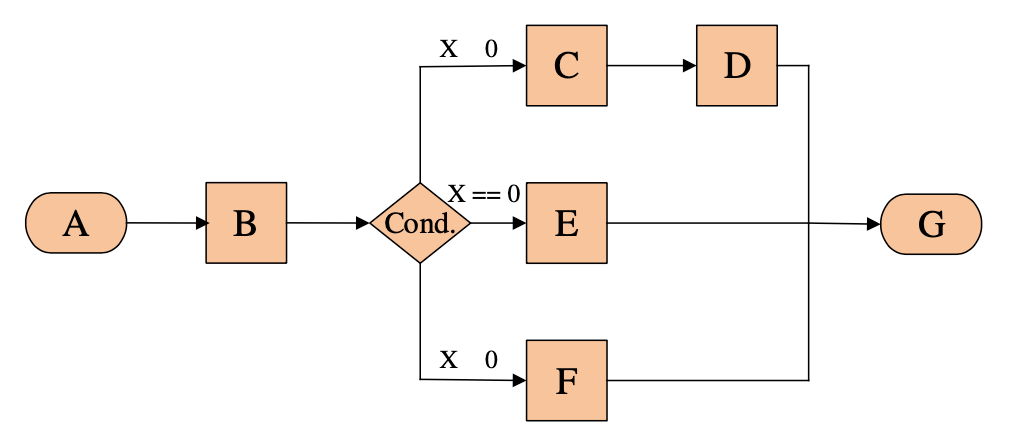
\includegraphics[scale=.5]{Figures/im}
		\caption{Execution flow example [3]}
	\end{figure}

	\noindent Accordingly, it can be realized that if n(*) denotes the number of logs for an event *, the following equations could be derived:
	
	\begin{center}
		n(A) = n(B)\\
		n(B) = n(C)+n(E)+n(F)\\
		n(C) = n(D)\\
		n(G) = n(D)+n(E)+n(F)\\
	\end{center}

	\noindent This series of equations represent the normal behavior of the system. Therefore, if any of this equations is not met as a timestamp, it should be concluded that there exists an anomaly in the system execution.
	
	\vspace{0.15cm}
	
	\noindent Invariants mining consists of three steps: first, singular value decomposition is used to create the invariant space, which calculates the number of invariants (r) that are needed to be mined; second, a brute force search method is used to find these r invariants; third, each mined invariant is validated by comparing its support value with a given threshold until r independent invariants are found.

	\vspace{0.6cm}
	\noindent \textbf{\Large Methodology}
	\vspace{0.5cm}
	
	\noindent The methodology for this report can be divided into two parts: 1. Log Parsing; 2. Feature Extraction and Anomaly Detection.
	
	\vspace{0.4cm}
	\noindent \textbf{\large 1. Log Parsing}
	\vspace{0.3cm}
	
	\noindent Log parsing is implemented by using logpai's logparser repository [4], which is available on GitHub. Python 2.7 was used to run the source code on a laptop, with a Quad-Core i7 CPU and 8GB of RAM. Each of the mentioned four models is evaluated on five widely-used datasets, each containing 2000 log messages: HDFS, Zookeeper, BGL, HPC, and Proxifier. The metrics for evaluation of these algorithms are calculated as below
	\begin{center}
		$Precision = \frac{\textmd{\# Accurate Pairs}}{\textmd{\# Parsed pairs}}$\\\vspace{0.2cm}
		
		$Recall = \frac{\textmd{\# Accurate Pairs}}{\textmd{\# Real pairs}}$\\\vspace{0.2cm}
		
		$F-score = 2*\frac{\textmd{Precision*Recall}}{\textmd{Precision+Recall}}$\\\vspace{0.2cm}
		
		$RandIndex = \frac{\textmd{\# Accurate Events (TN+TP)}}{\textmd{\# Ground truth (TN+FN+TP+FP)}} \textmd{ [3]}$\\\vspace{0.2cm}
		
		$Runtime = \textmd{End Time - Start Time (in Seconds)}$
	\end{center}
	
	
	\vspace{0.4cm}
	\noindent \textbf{\large 2. Feature Extraction and Anomaly Detection}
	\vspace{0.3cm}
	
	\noindent Feature extraction and anomaly detection is implemented by using logpai's loglizer repository [5], which is also available on GitHub. Python 3.8 was used to run the source code on the same system. Due to its performance, which will be discussed in the next section, the IPLoM method was used to parse the provided HDFS logs. Accordingly, the mentioned two anomaly detection methods PCA and Invariants mining were implemented and evaluated, given that 80\% of the data was used for training and the rest was used for testing. The metrics for evaluation of these two algorithms are calculated as below
	\begin{center}
		$Precision = \frac{\textmd{\# Anomalies Detected}}{\textmd{\# Anomalies Reported}}$\\\vspace{0.2cm}
		
		$Recall = \frac{\textmd{\# Anomalies Detected}}{\textmd{\# All Anomalies}}$\\\vspace{0.2cm}
		
		$F-score = 2*\frac{\textmd{Precision*Recall}}{\textmd{Precision+Recall}}$\\\vspace{0.2cm}
		
		$Runtime = \textmd{End Time - Start Time (in Seconds)}$
	\end{center}

	\noindent 
	
	\vspace{0.6cm}
	\noindent \textbf{\Large Results and Discussion}
	\vspace{0.5cm}
	
	\noindent Similar to the previous parts, the section is divided into two parts:  1. Log Parsing; 2. Feature Extraction and Anomaly Detection.
	
	\vspace{0.4cm}
	\noindent \textbf{\large 1. Log Parsing}
	\vspace{0.3cm}
	
	\noindent The performance of the four log parsing algorithms on the mentioned five datasets based on each of the three required evaluation metrics (F-score, RandIndex, and Runtime) are illustrated respectively below:
	
	\vspace{-0.5cm}
	\begin{figure}[H]
		\centering
		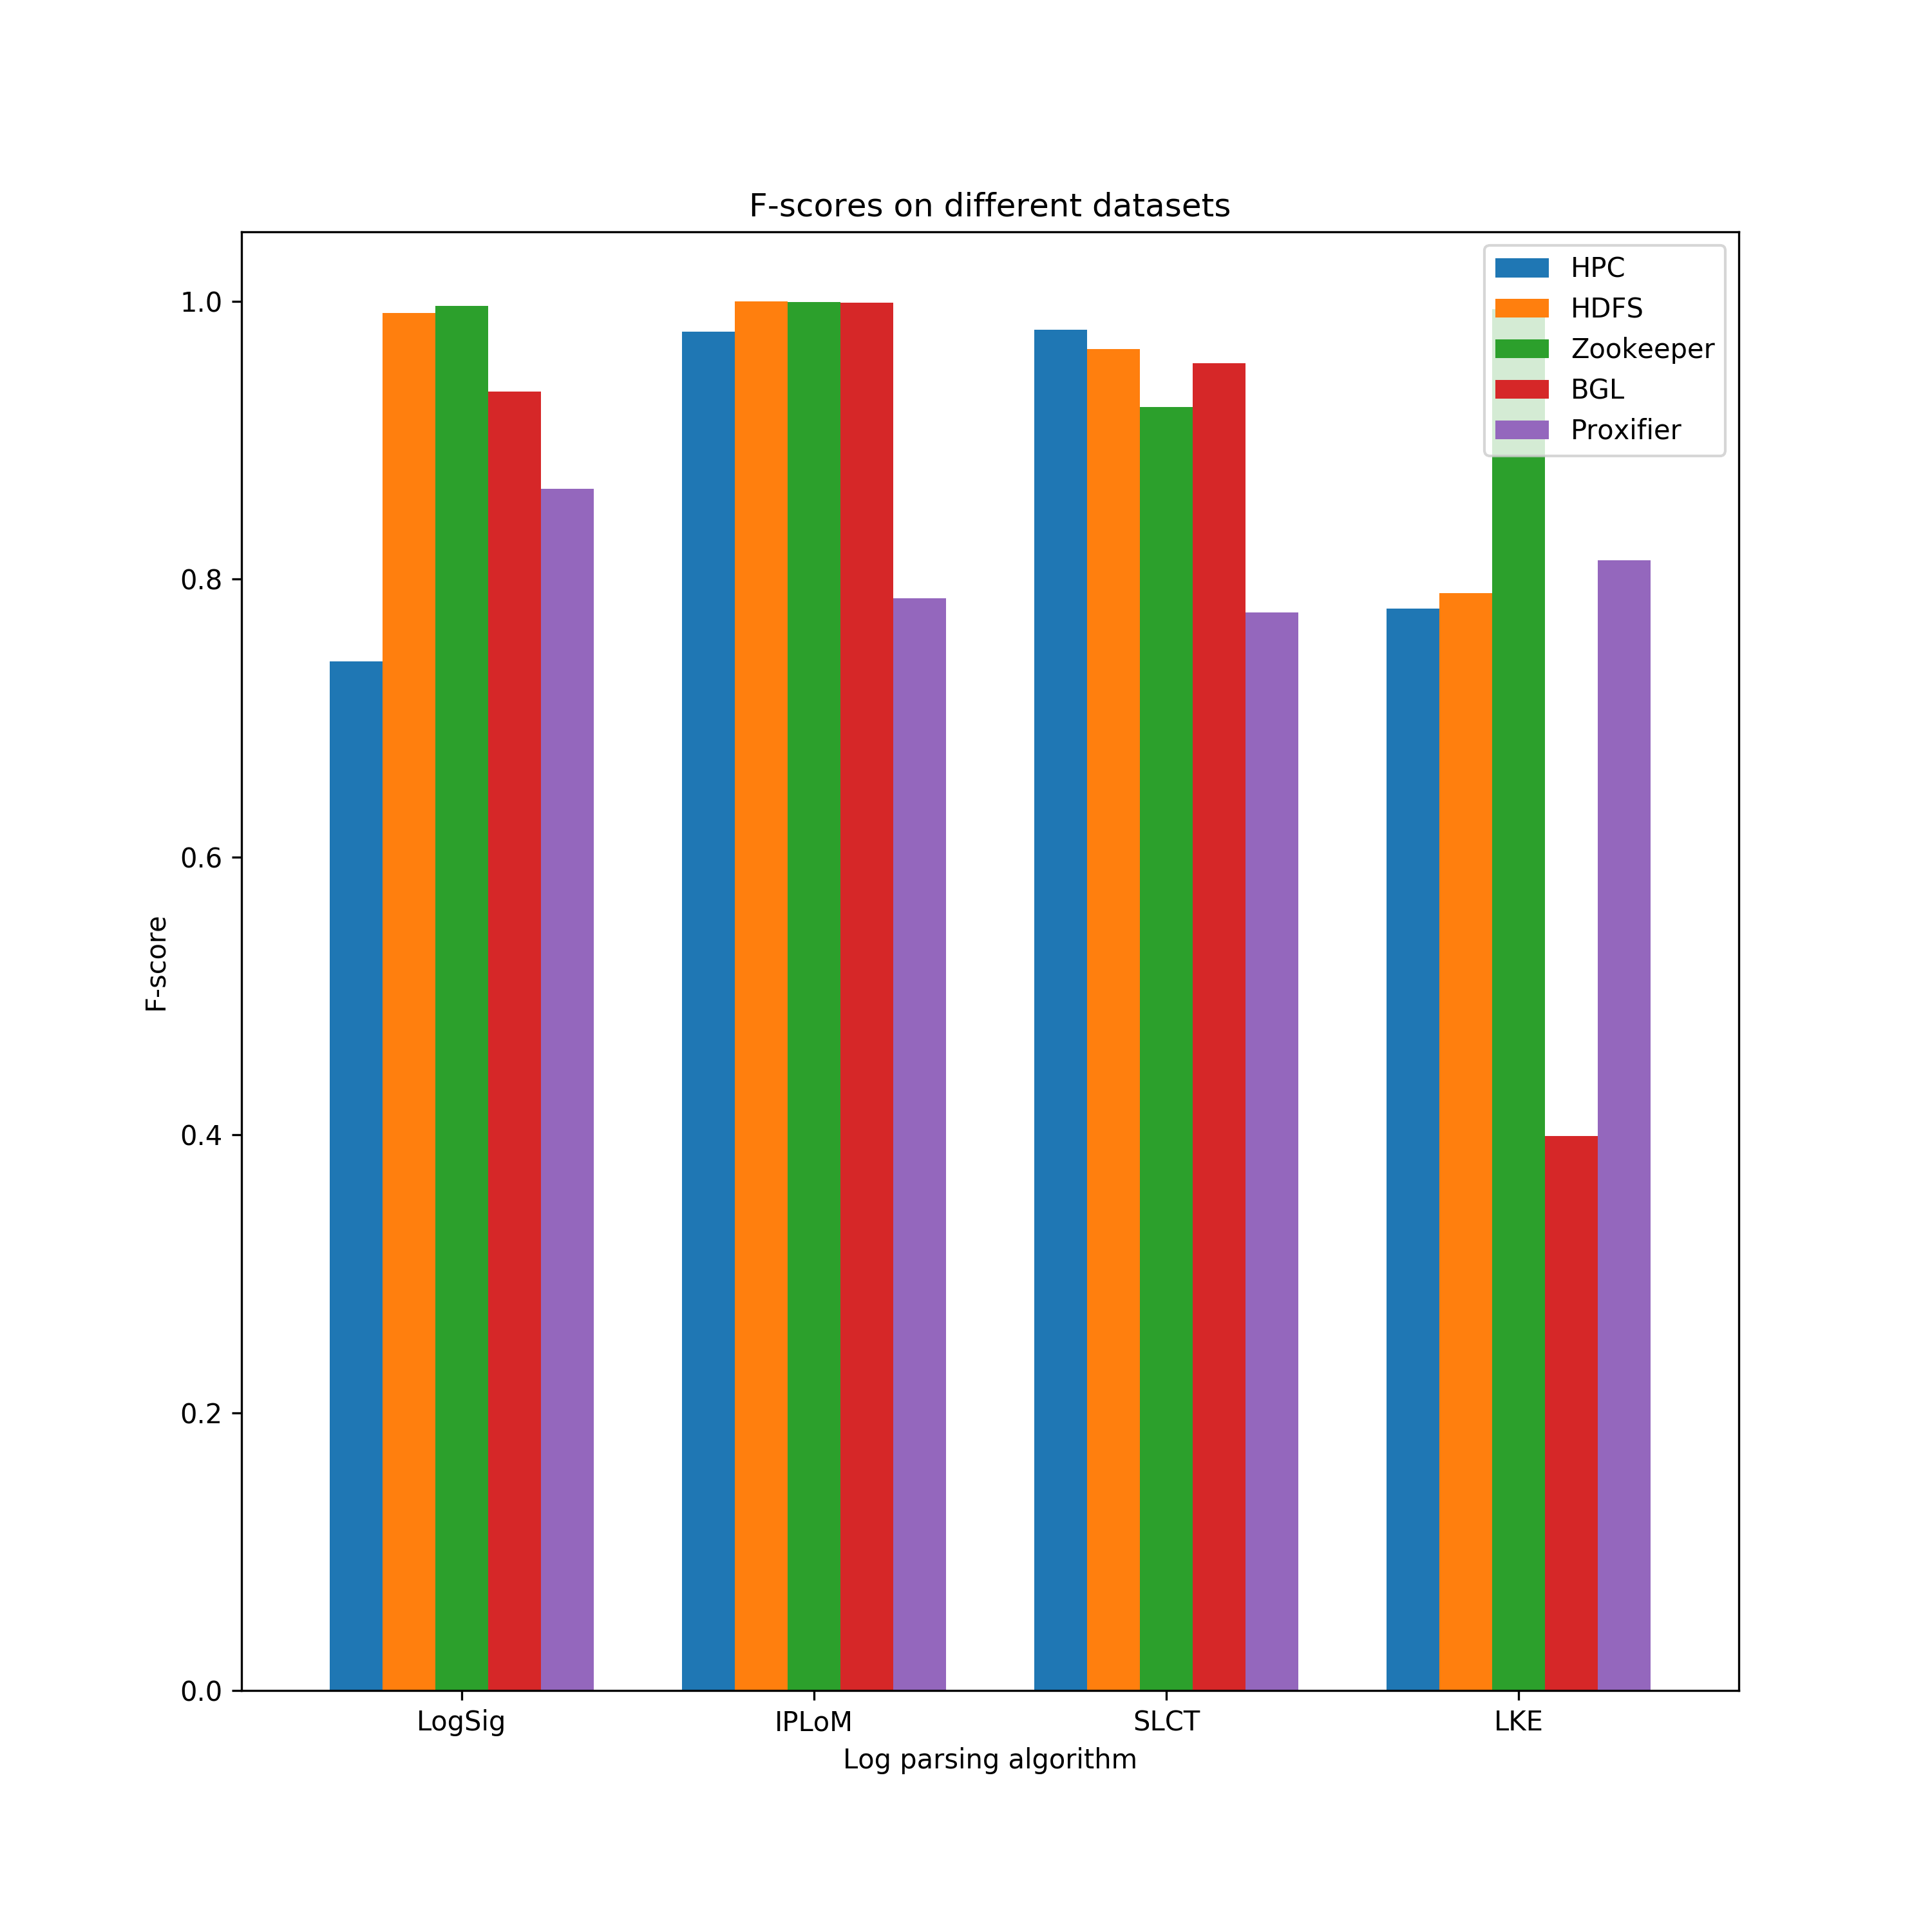
\includegraphics[width=13cm, height=7.7cm]{Figures/F1_1}
		\vspace{-0.8cm}
		
		\caption{F-Score Evaluation Results for Different Datasets}
	\end{figure}
	
	\vspace{-1cm}
	\begin{figure}[H]
		\centering
		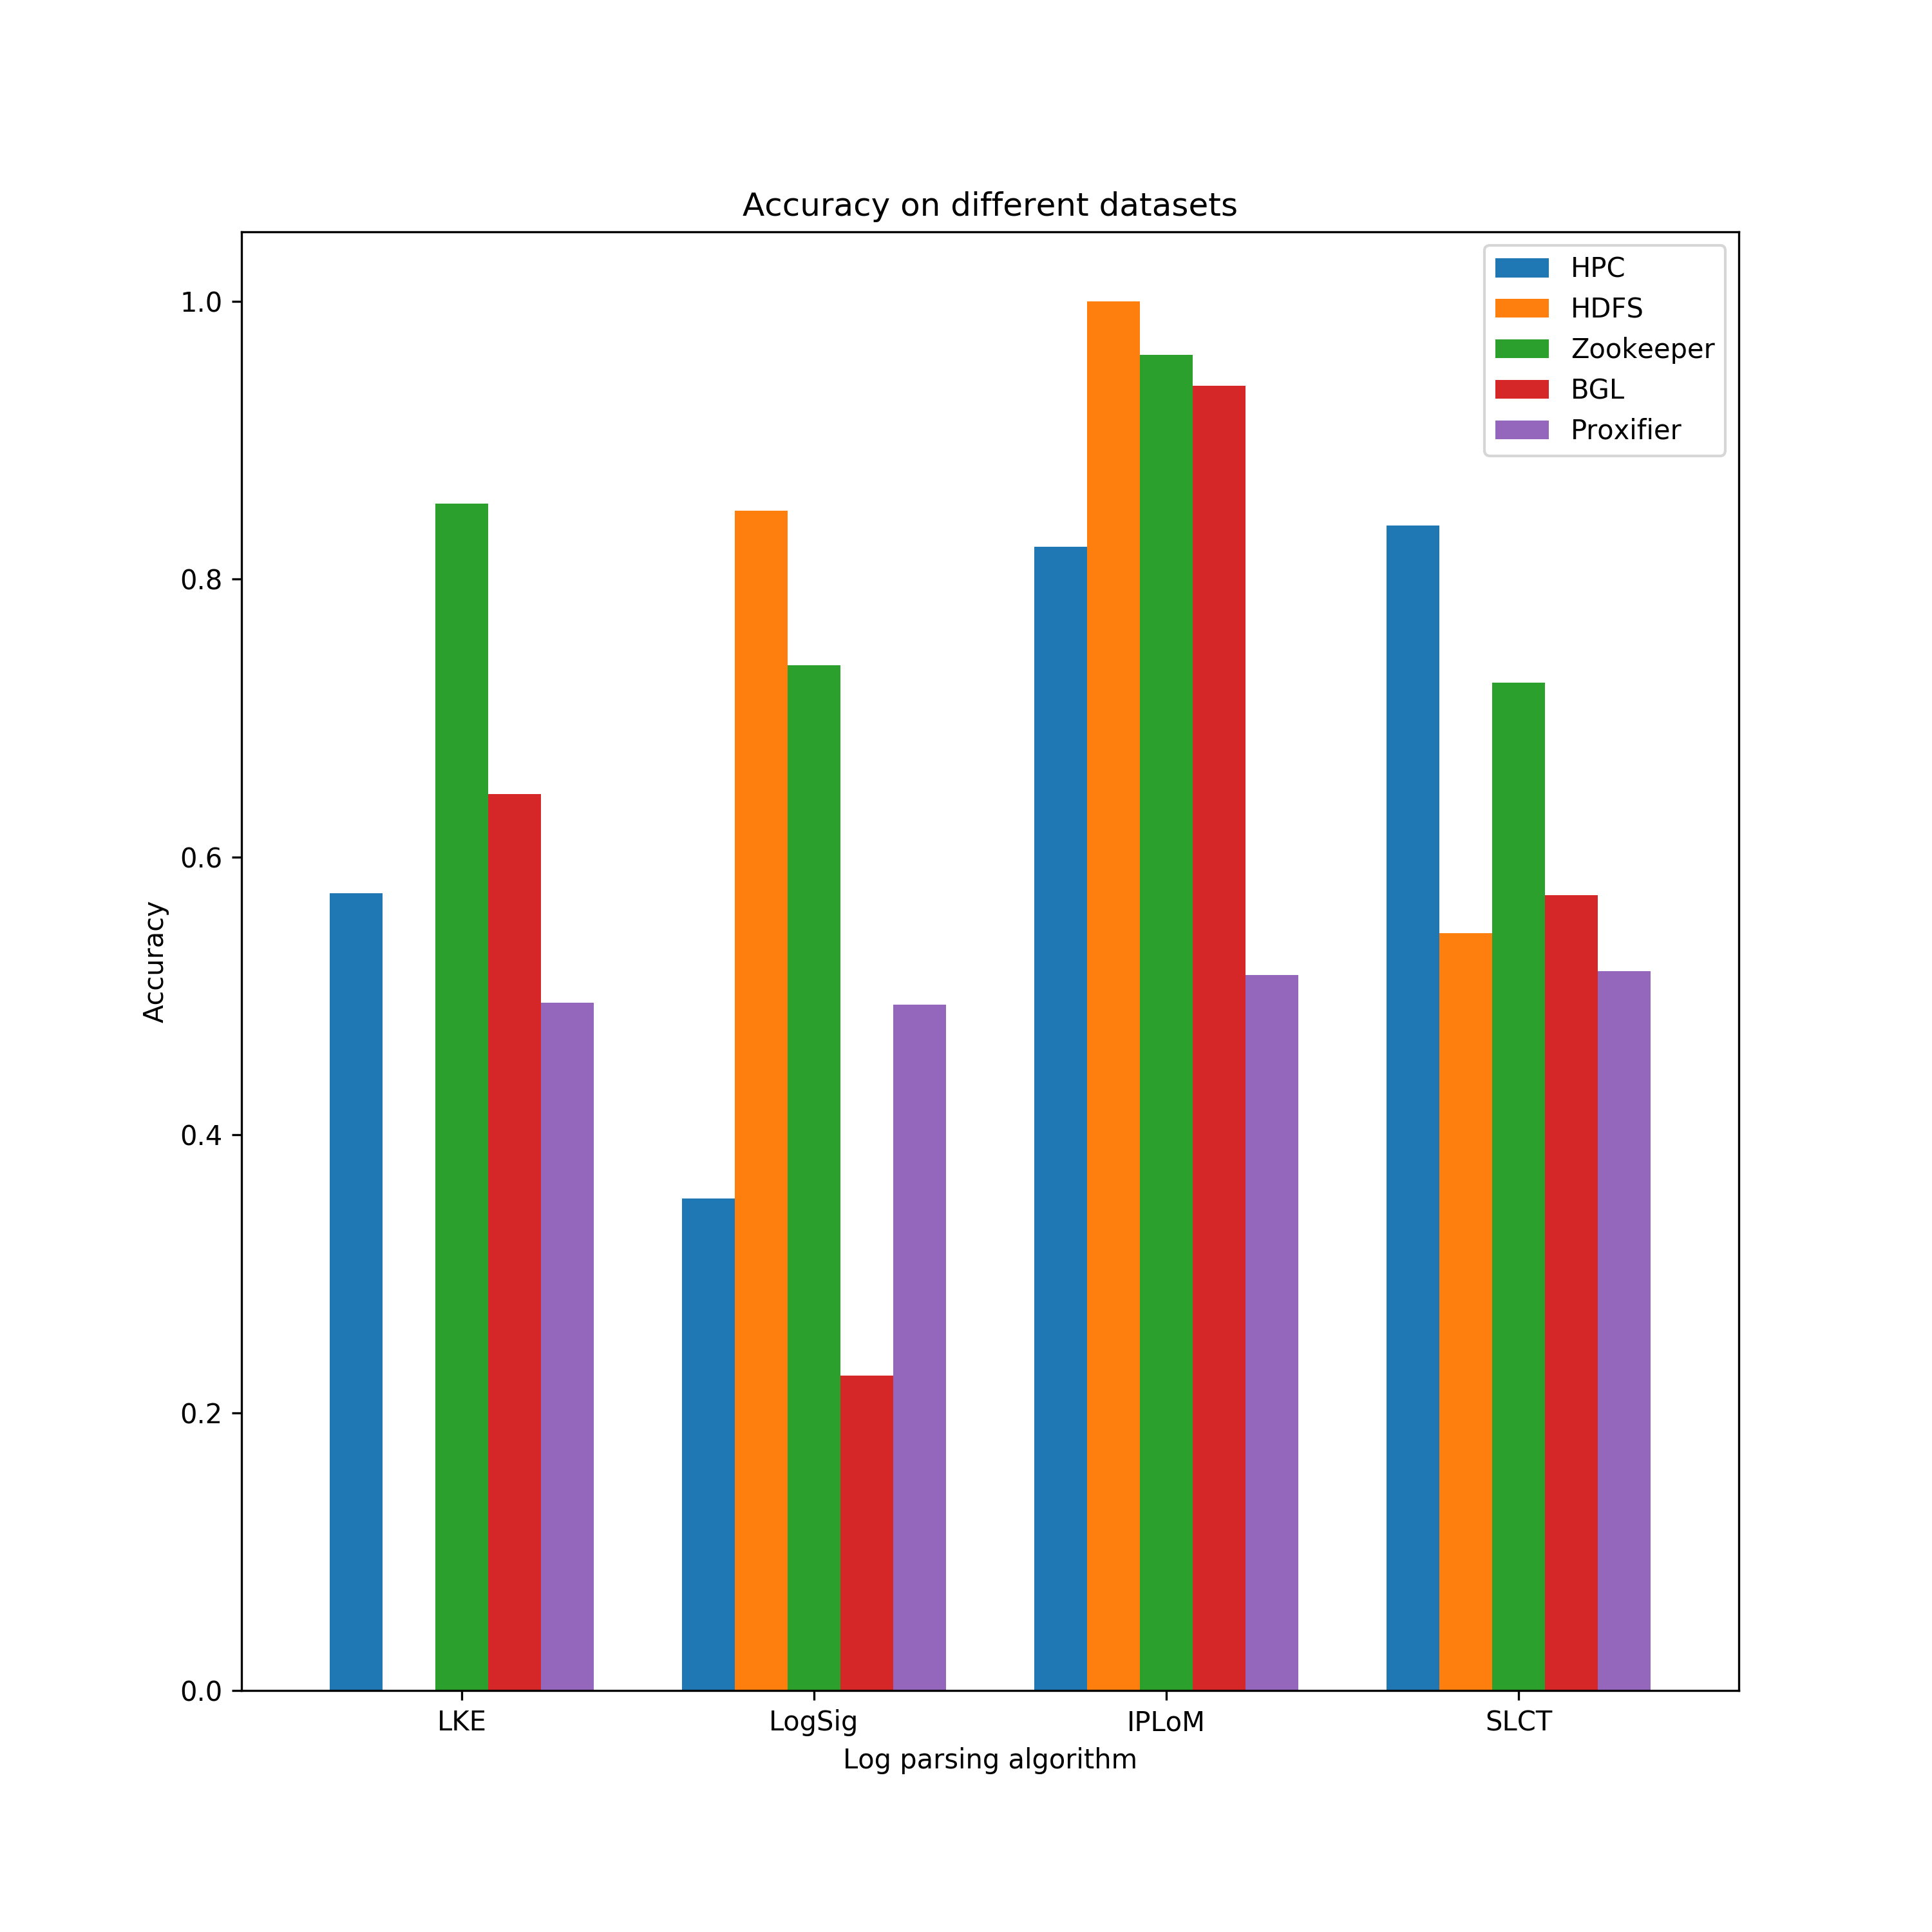
\includegraphics[width=13cm, height=7.7cm]{Figures/ACC_1}
		\vspace{-0.8cm}
		
		\caption{RandIndex Evaluation Results for Different Datasets}
	\end{figure}

	\begin{figure}[H]
		\centering
		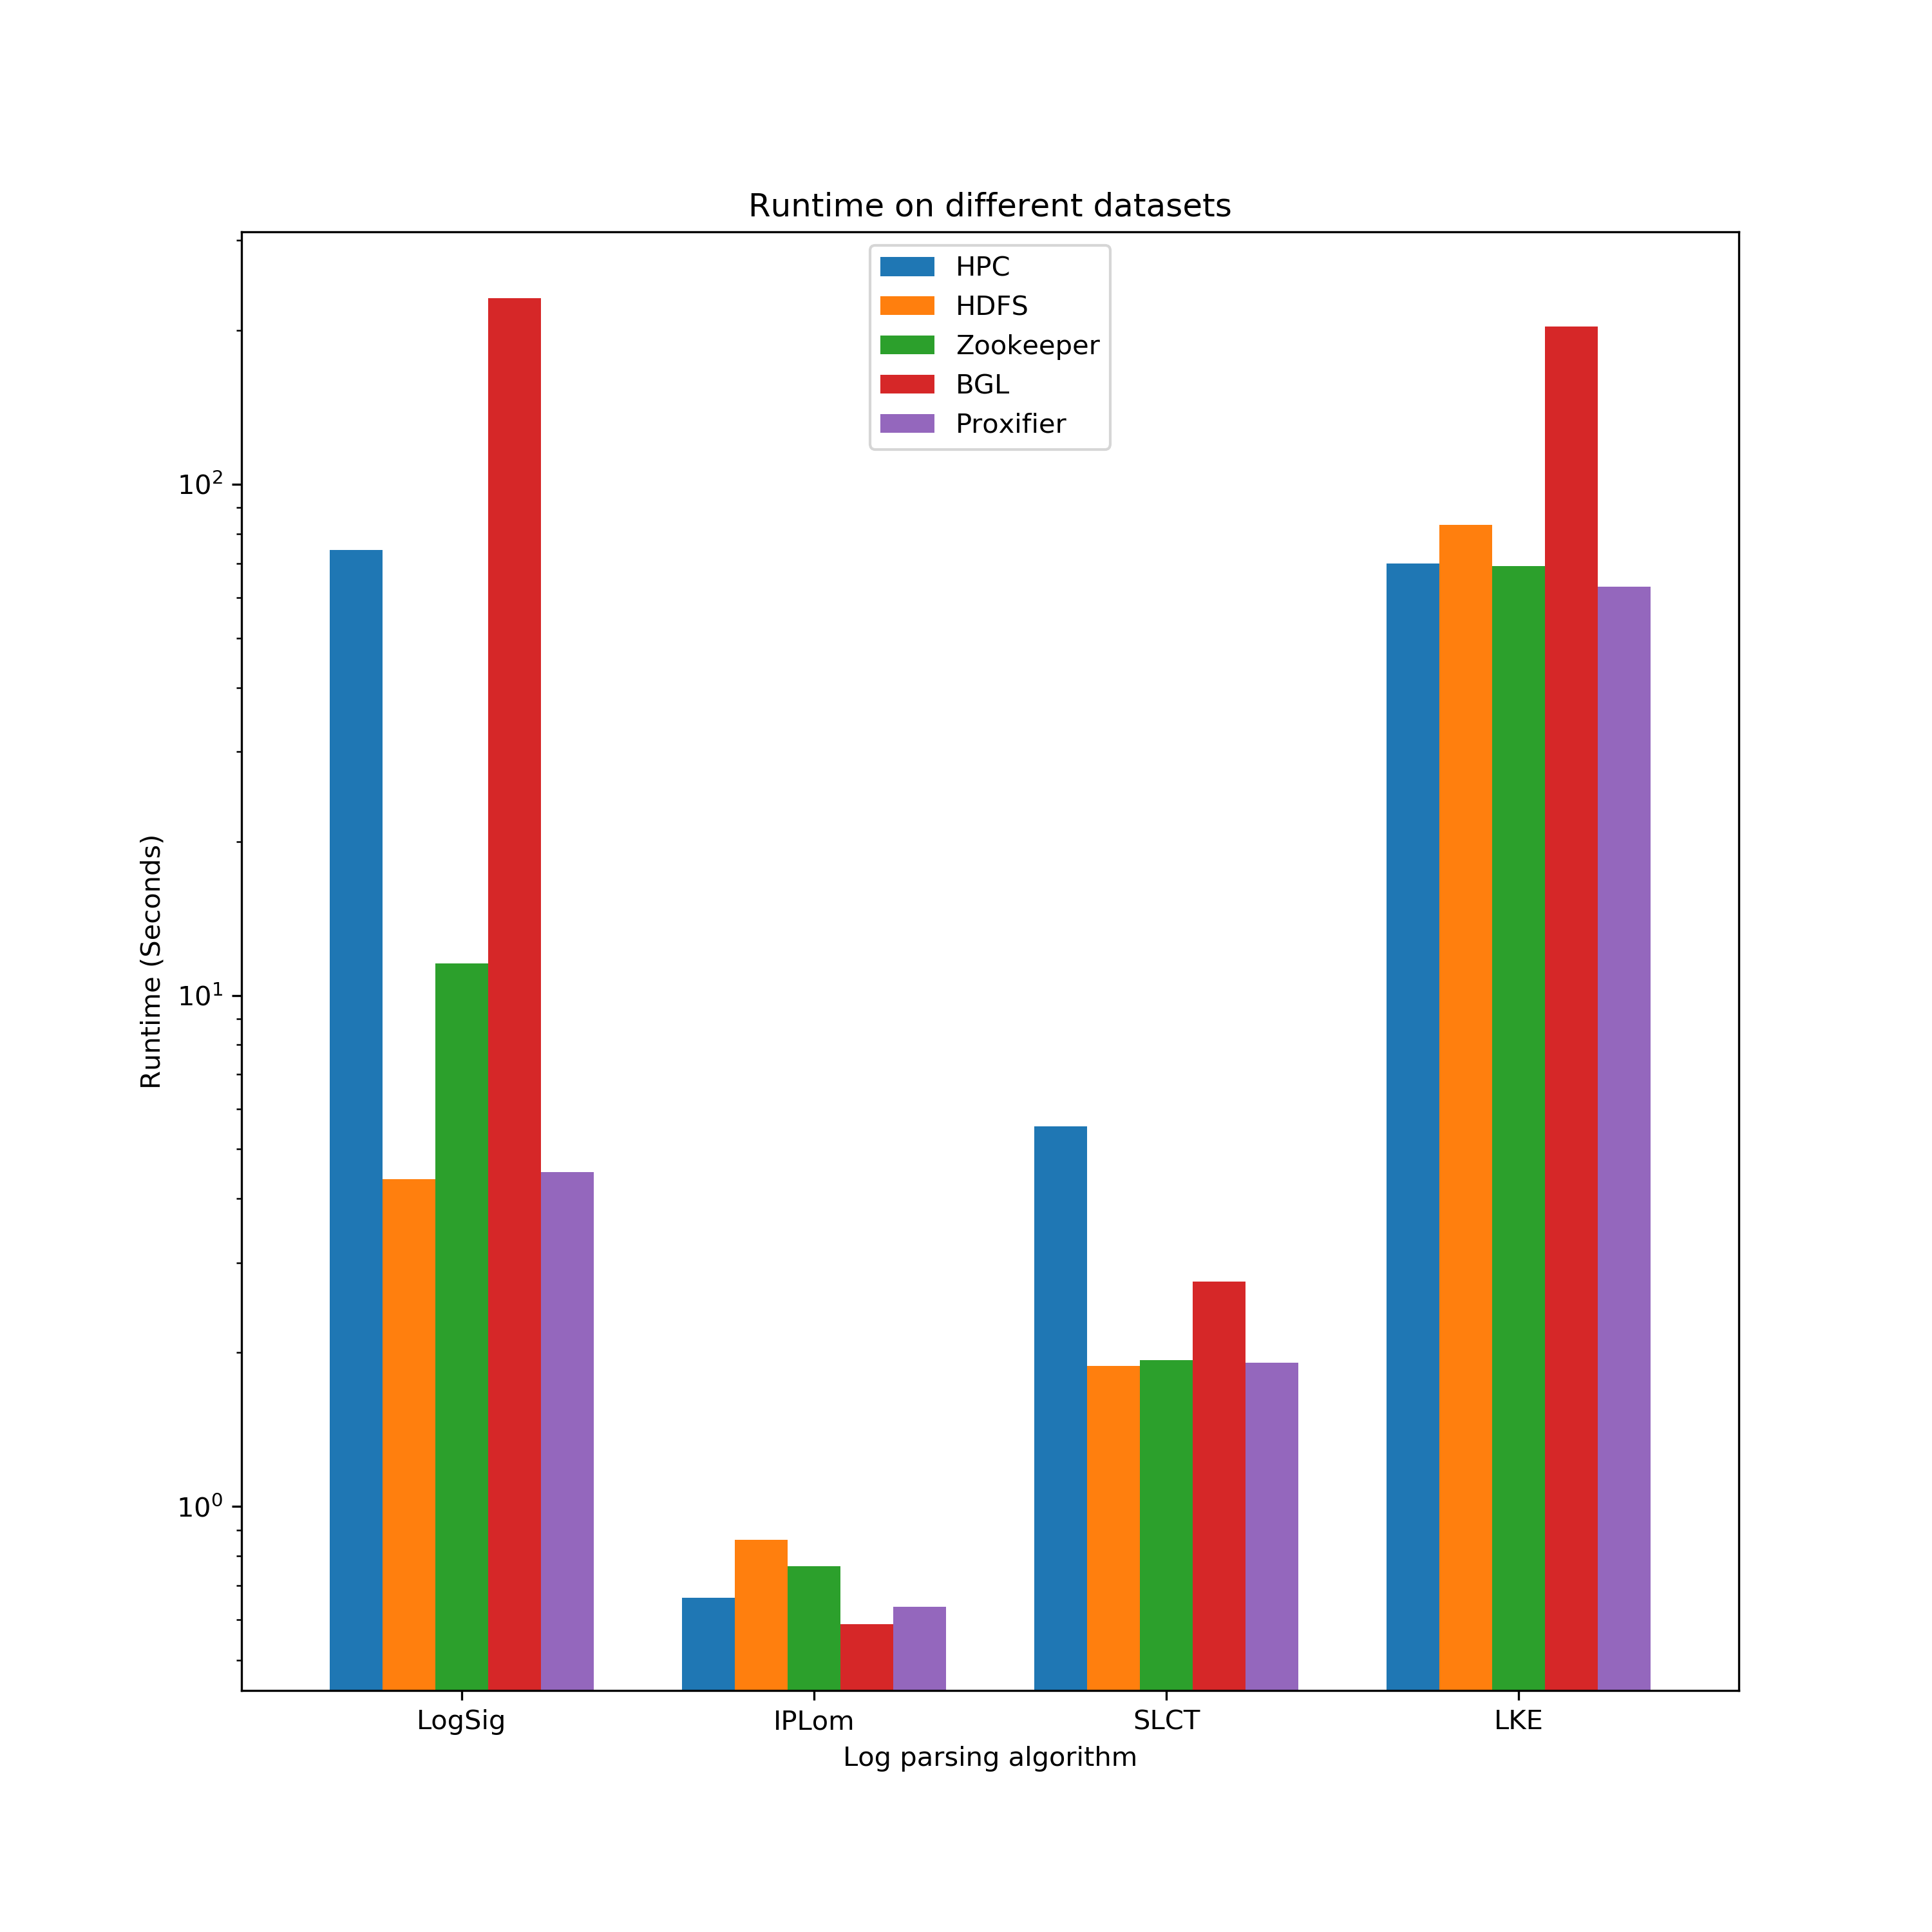
\includegraphics[width=13cm, height=7.7cm]{Figures/Runtime_1}
		\vspace{-0.8cm}
		
		\caption{Runtime Evaluation Results for Different Datasets}
	\end{figure}


	\noindent As displayed in the above figures, it can be observed that the runtime of LKE and LogSig is comparatively long, with LKE's longtime being the longest; this is a major disadvantage in comparison to the other available log parsing methods as it makes the experience of observing and fine-tuning the parameters fairly challenging and time consuming (check Limitations). Figures 2 and 3 also demonstrate that the performance of these two algorithms is much lower on the HPC and BGL datasets; this behavior is expected as these two datasets have a comparatively larger length and more event types and therefore, there is more room for error when using clustering-based algorithms such as LKE and LogSig.
	
	
	\noindent In addition, it can be observed that IPLoM achieves the highest overall accuracy as well as F-score on the HDFS dataset while performing within the lowest runtime for all datasets among the four discussed algorithms; these two factors are considered as this method's biggest advantages. Considering the runtime, Figure 4 shows that SLCT parses the log messages in a rather short running time. Hence, it can be derived that the heuristic rules regarding the characteristics of the log messages are not only essential for producing accurate log parsing but also are necessary for obtaining a linear time complexity. 
	
	\vspace{0.4cm}
	\noindent \textbf{\large 2. Feature Extraction and Anomaly Detection}
	\vspace{0.3cm}

	\noindent Based on the results of the previous section, IPLoM was used to parse the full HDFS dataset. Accordingly, the features of the parsed logs were extracted and the performance of PCA and Invariants Mining on the given events count matrix based on each of the required metrics (F-score, Precision, Recall, and Runtime) were recorded. The corresponding figures are displayed respectively below:
	
	\begin{figure}[H]
		\centering
		\begin{subfigure}[H]{0.45\textwidth}
			\centering
			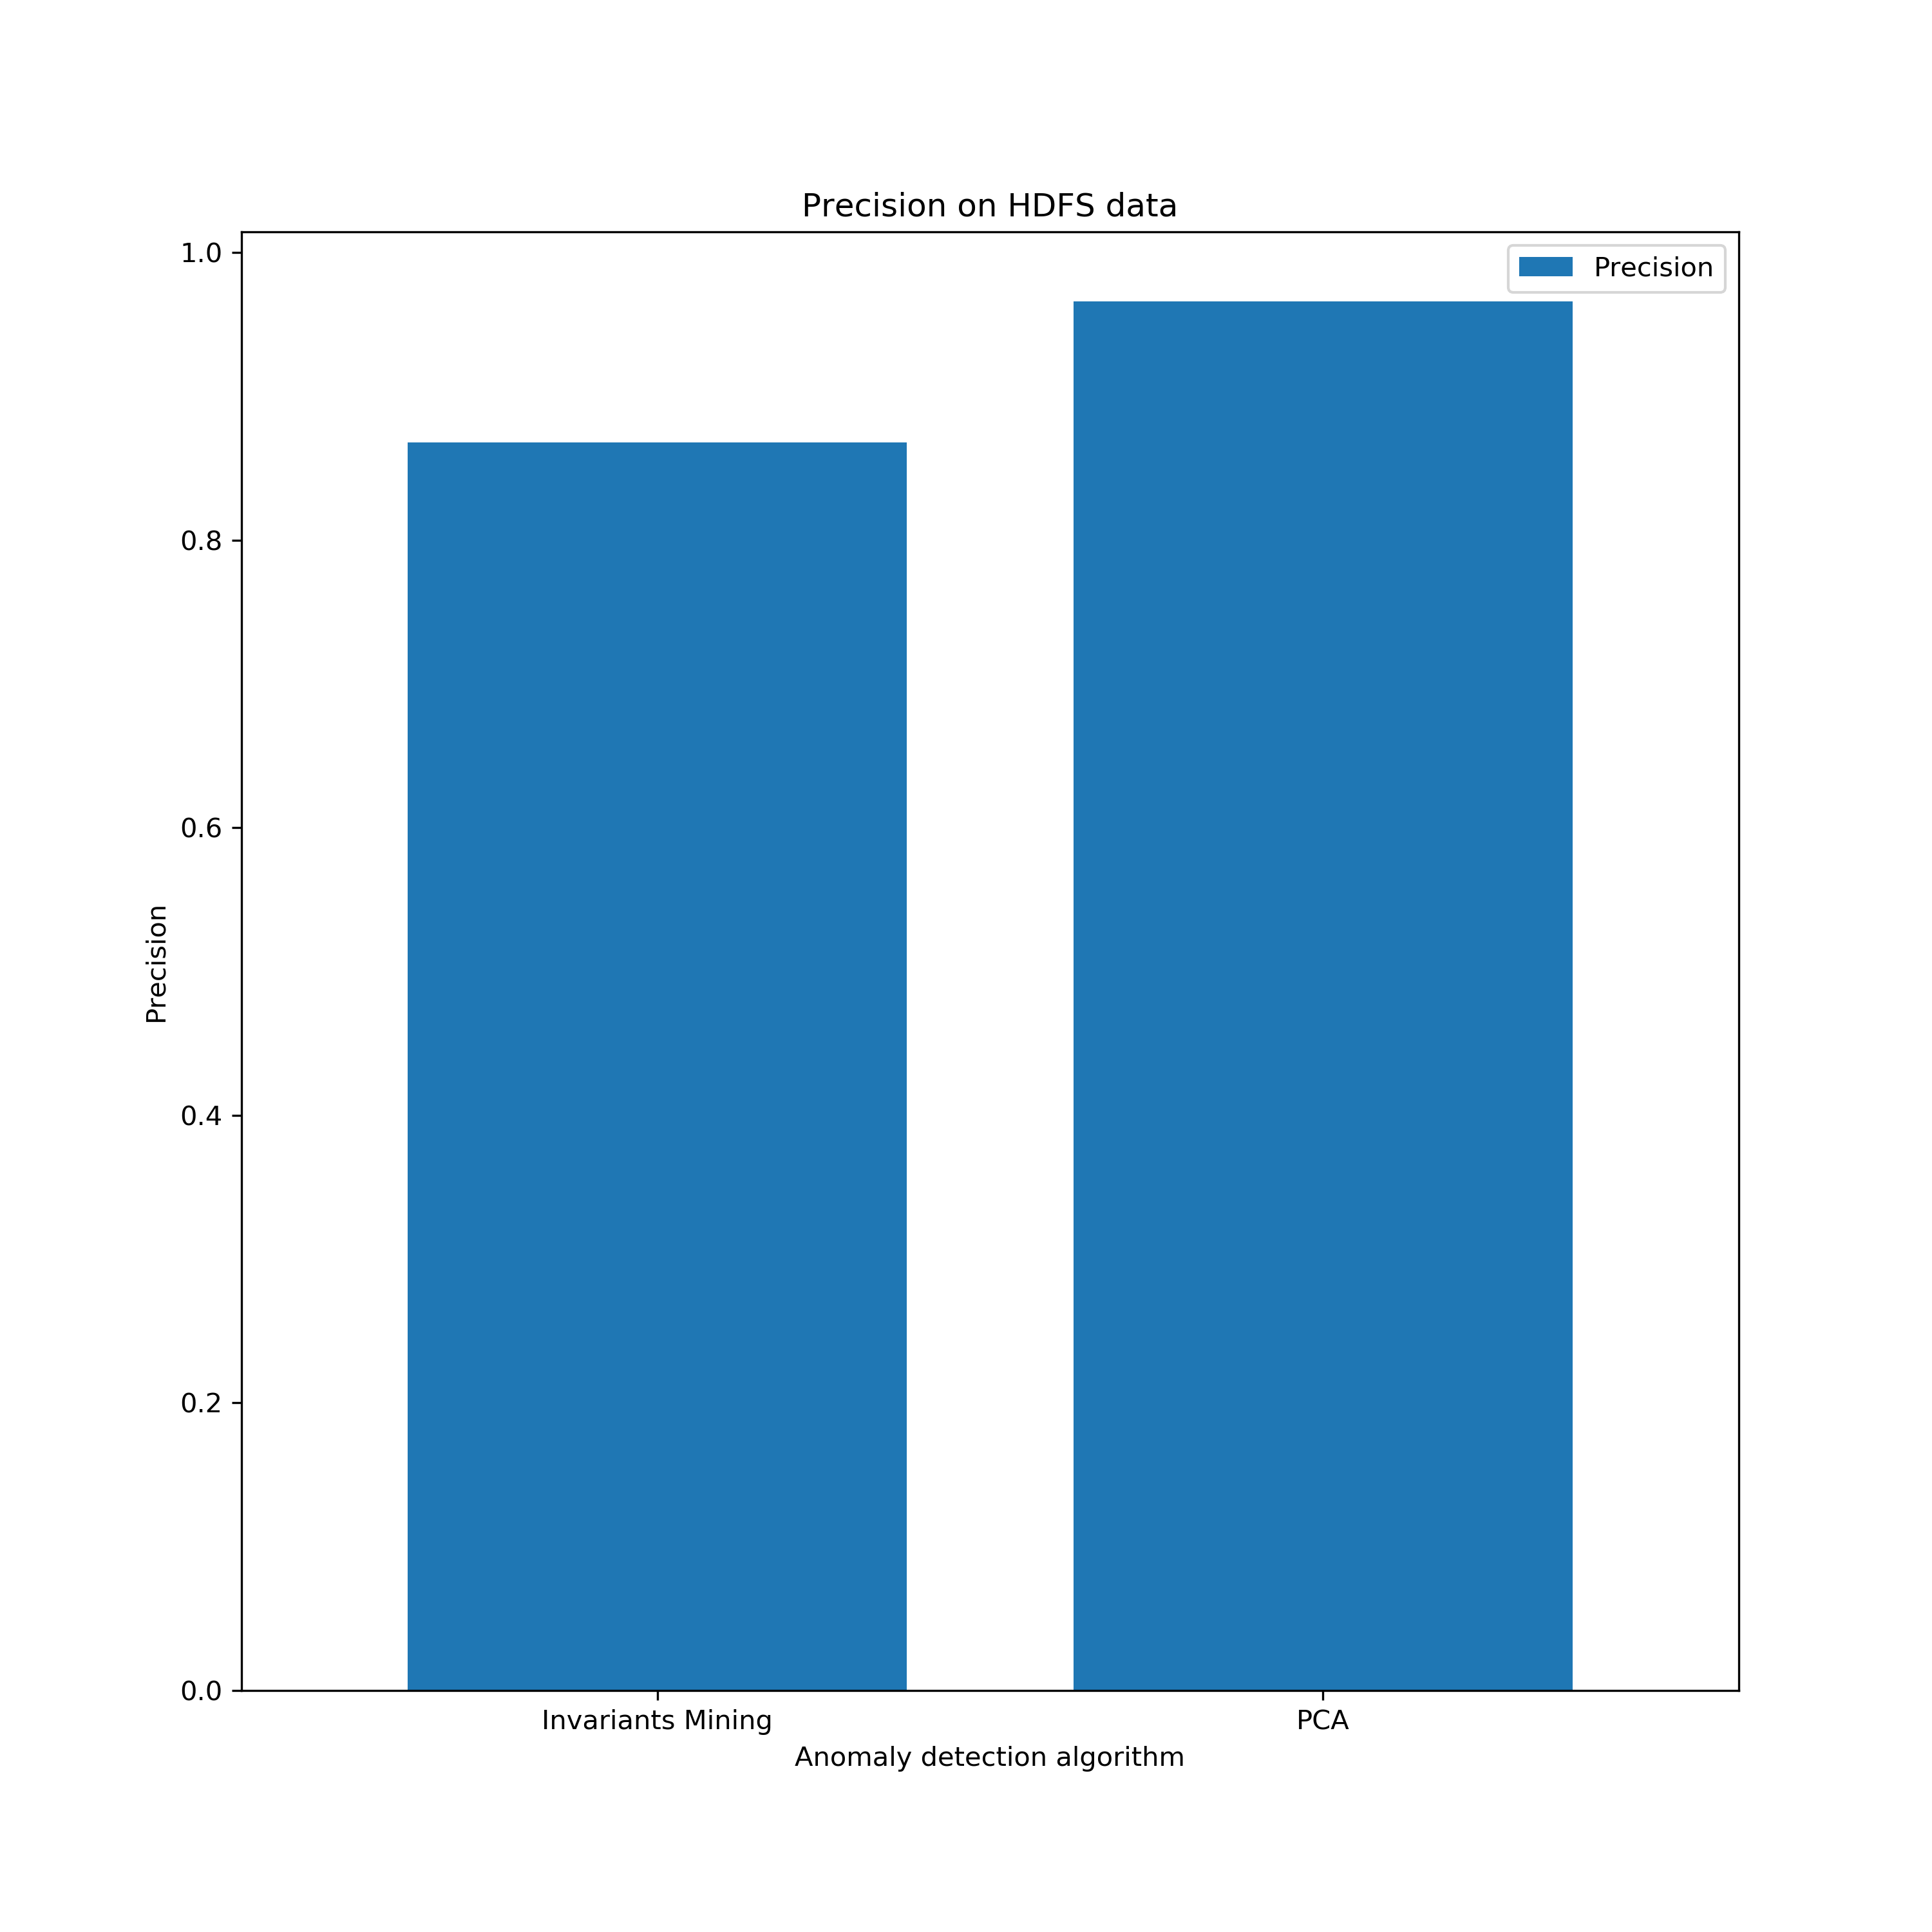
\includegraphics[width=1.3\textwidth]{Figures/Precision_2}
			
			\vspace{-0.3cm}
			\caption{Training data}
		\end{subfigure}
		\hfill
		\begin{subfigure}[H]{0.45\textwidth}
			\centering
			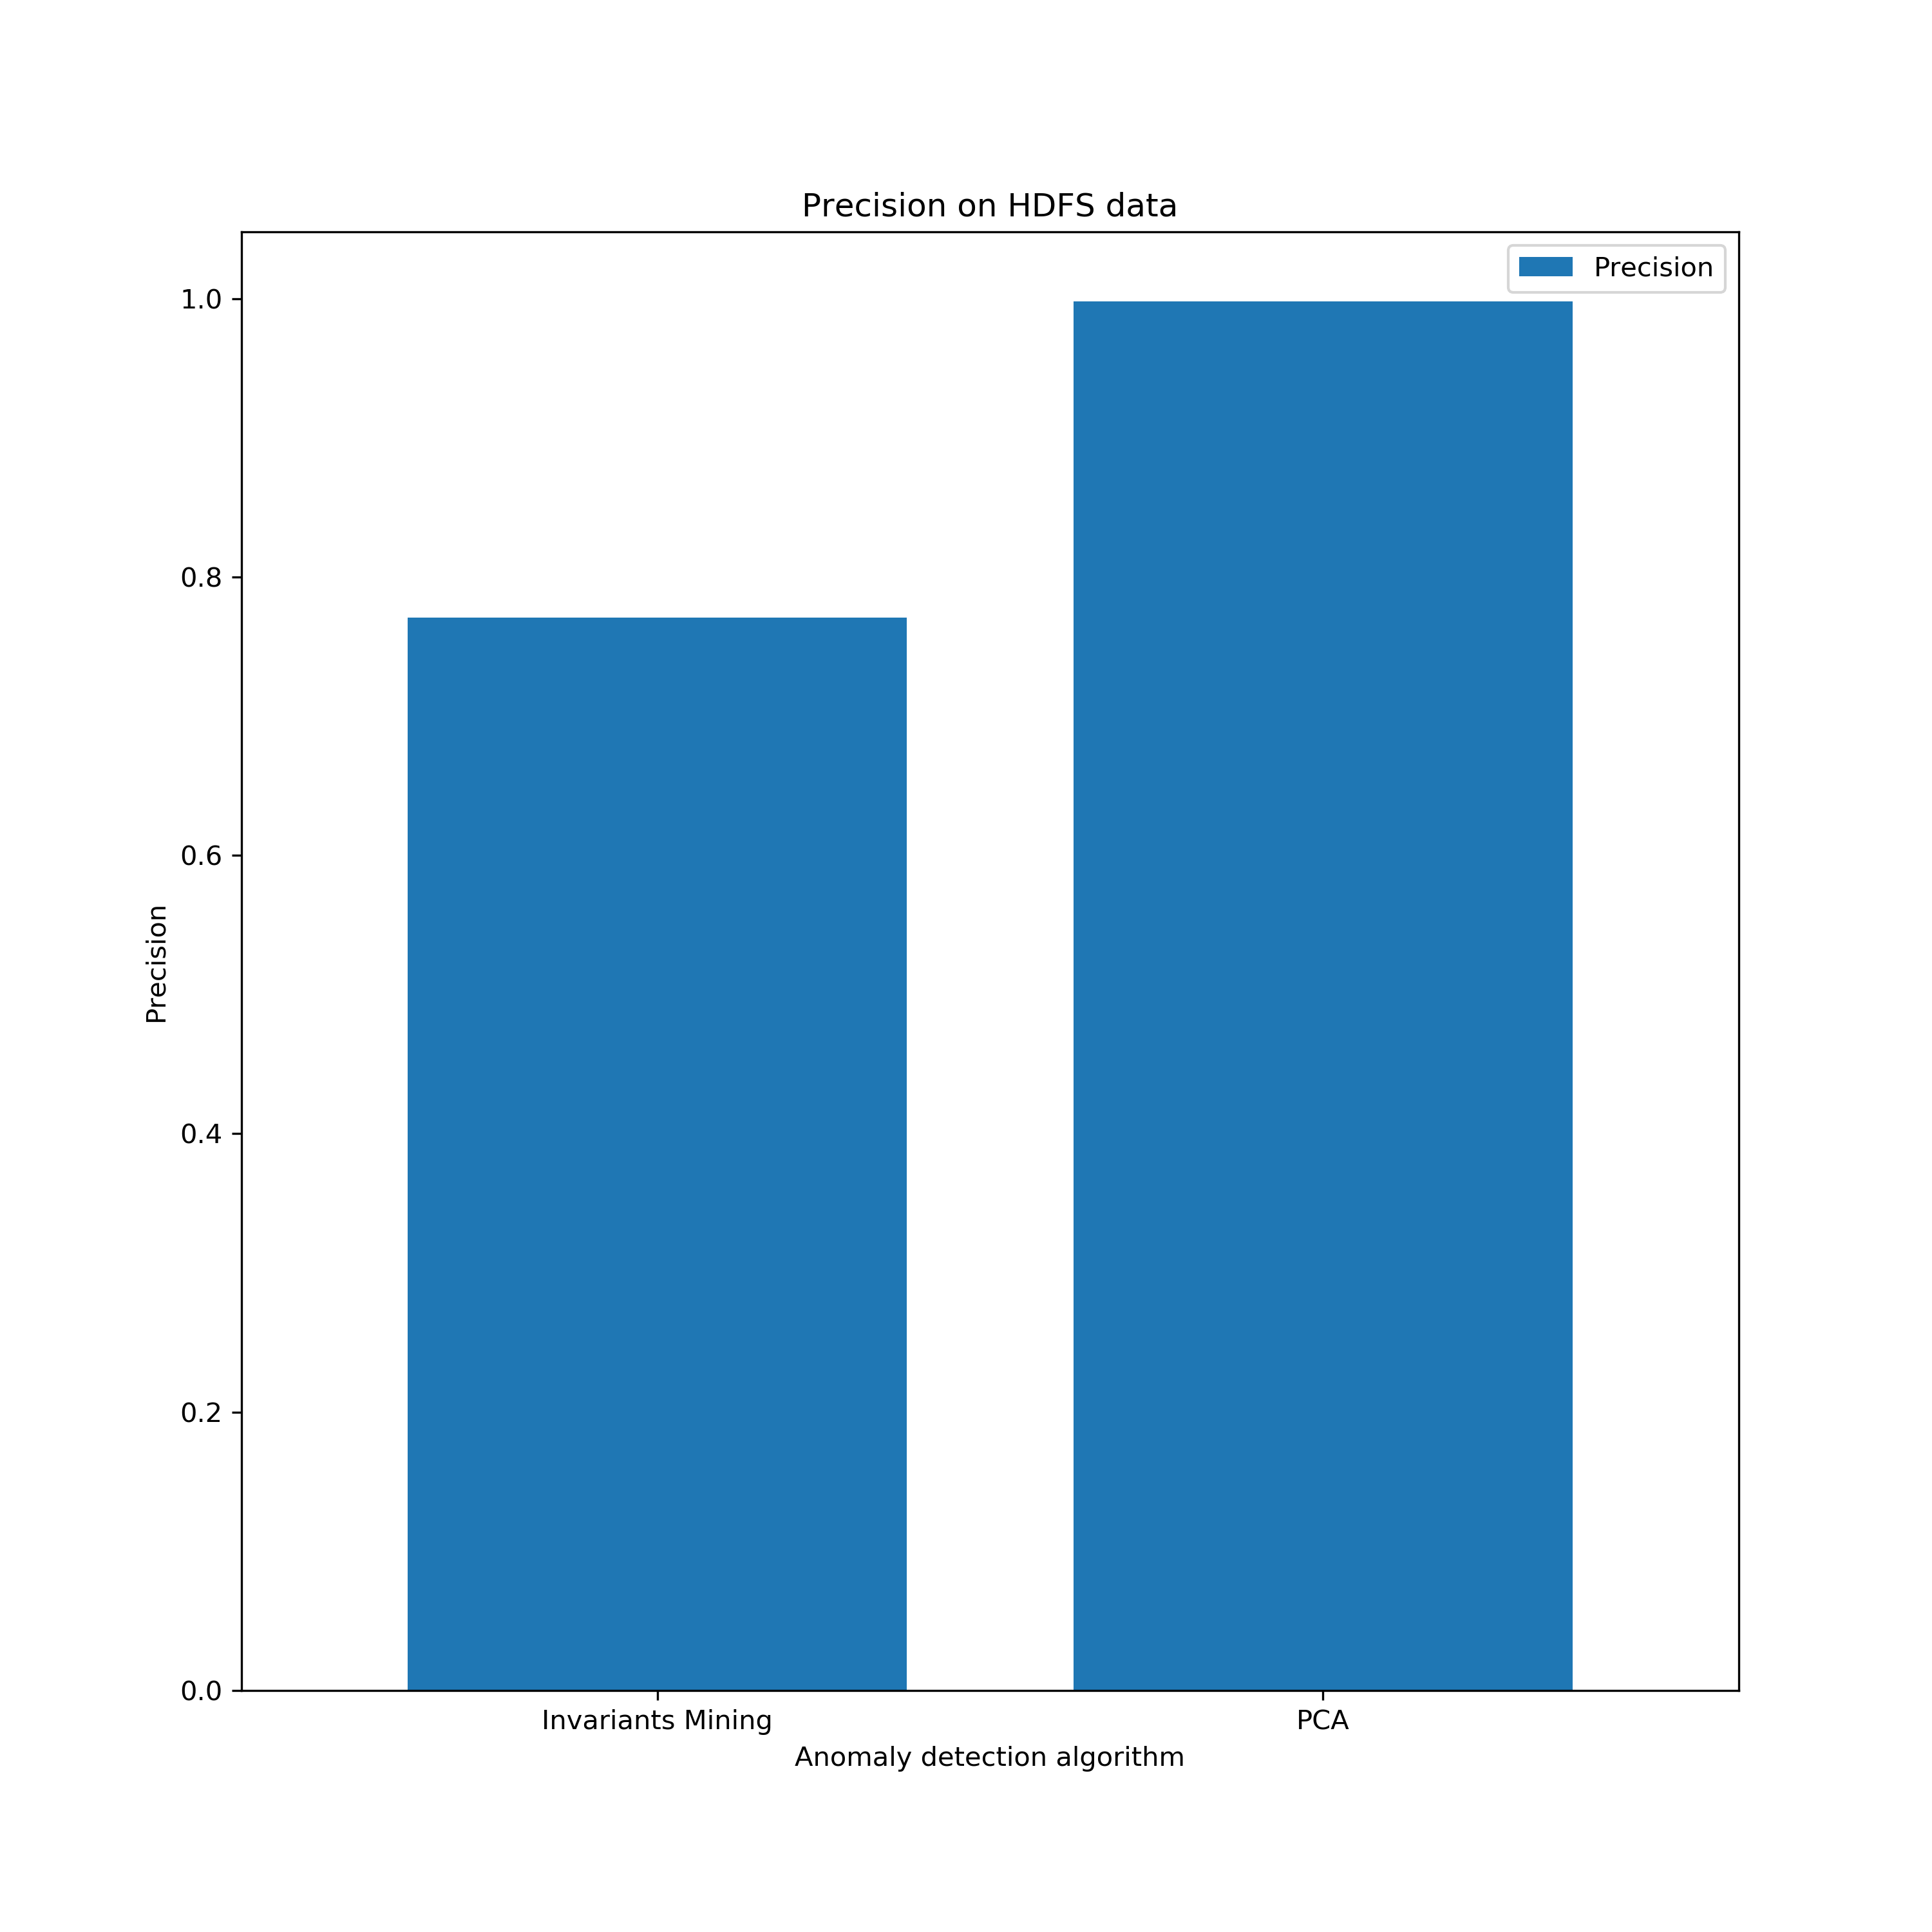
\includegraphics[width=1.3\textwidth]{Figures/Precision_2_test}
			
			\vspace{-0.3cm}
			\caption{Testing data}
		\end{subfigure}
		\vspace{-0.1cm}
		\caption{Precision evaluation results for HDFS data}
	\end{figure}

	\vspace{-0.4cm}
	\begin{figure}[H]
		\centering
		\begin{subfigure}[H]{0.45\textwidth}
			\centering
			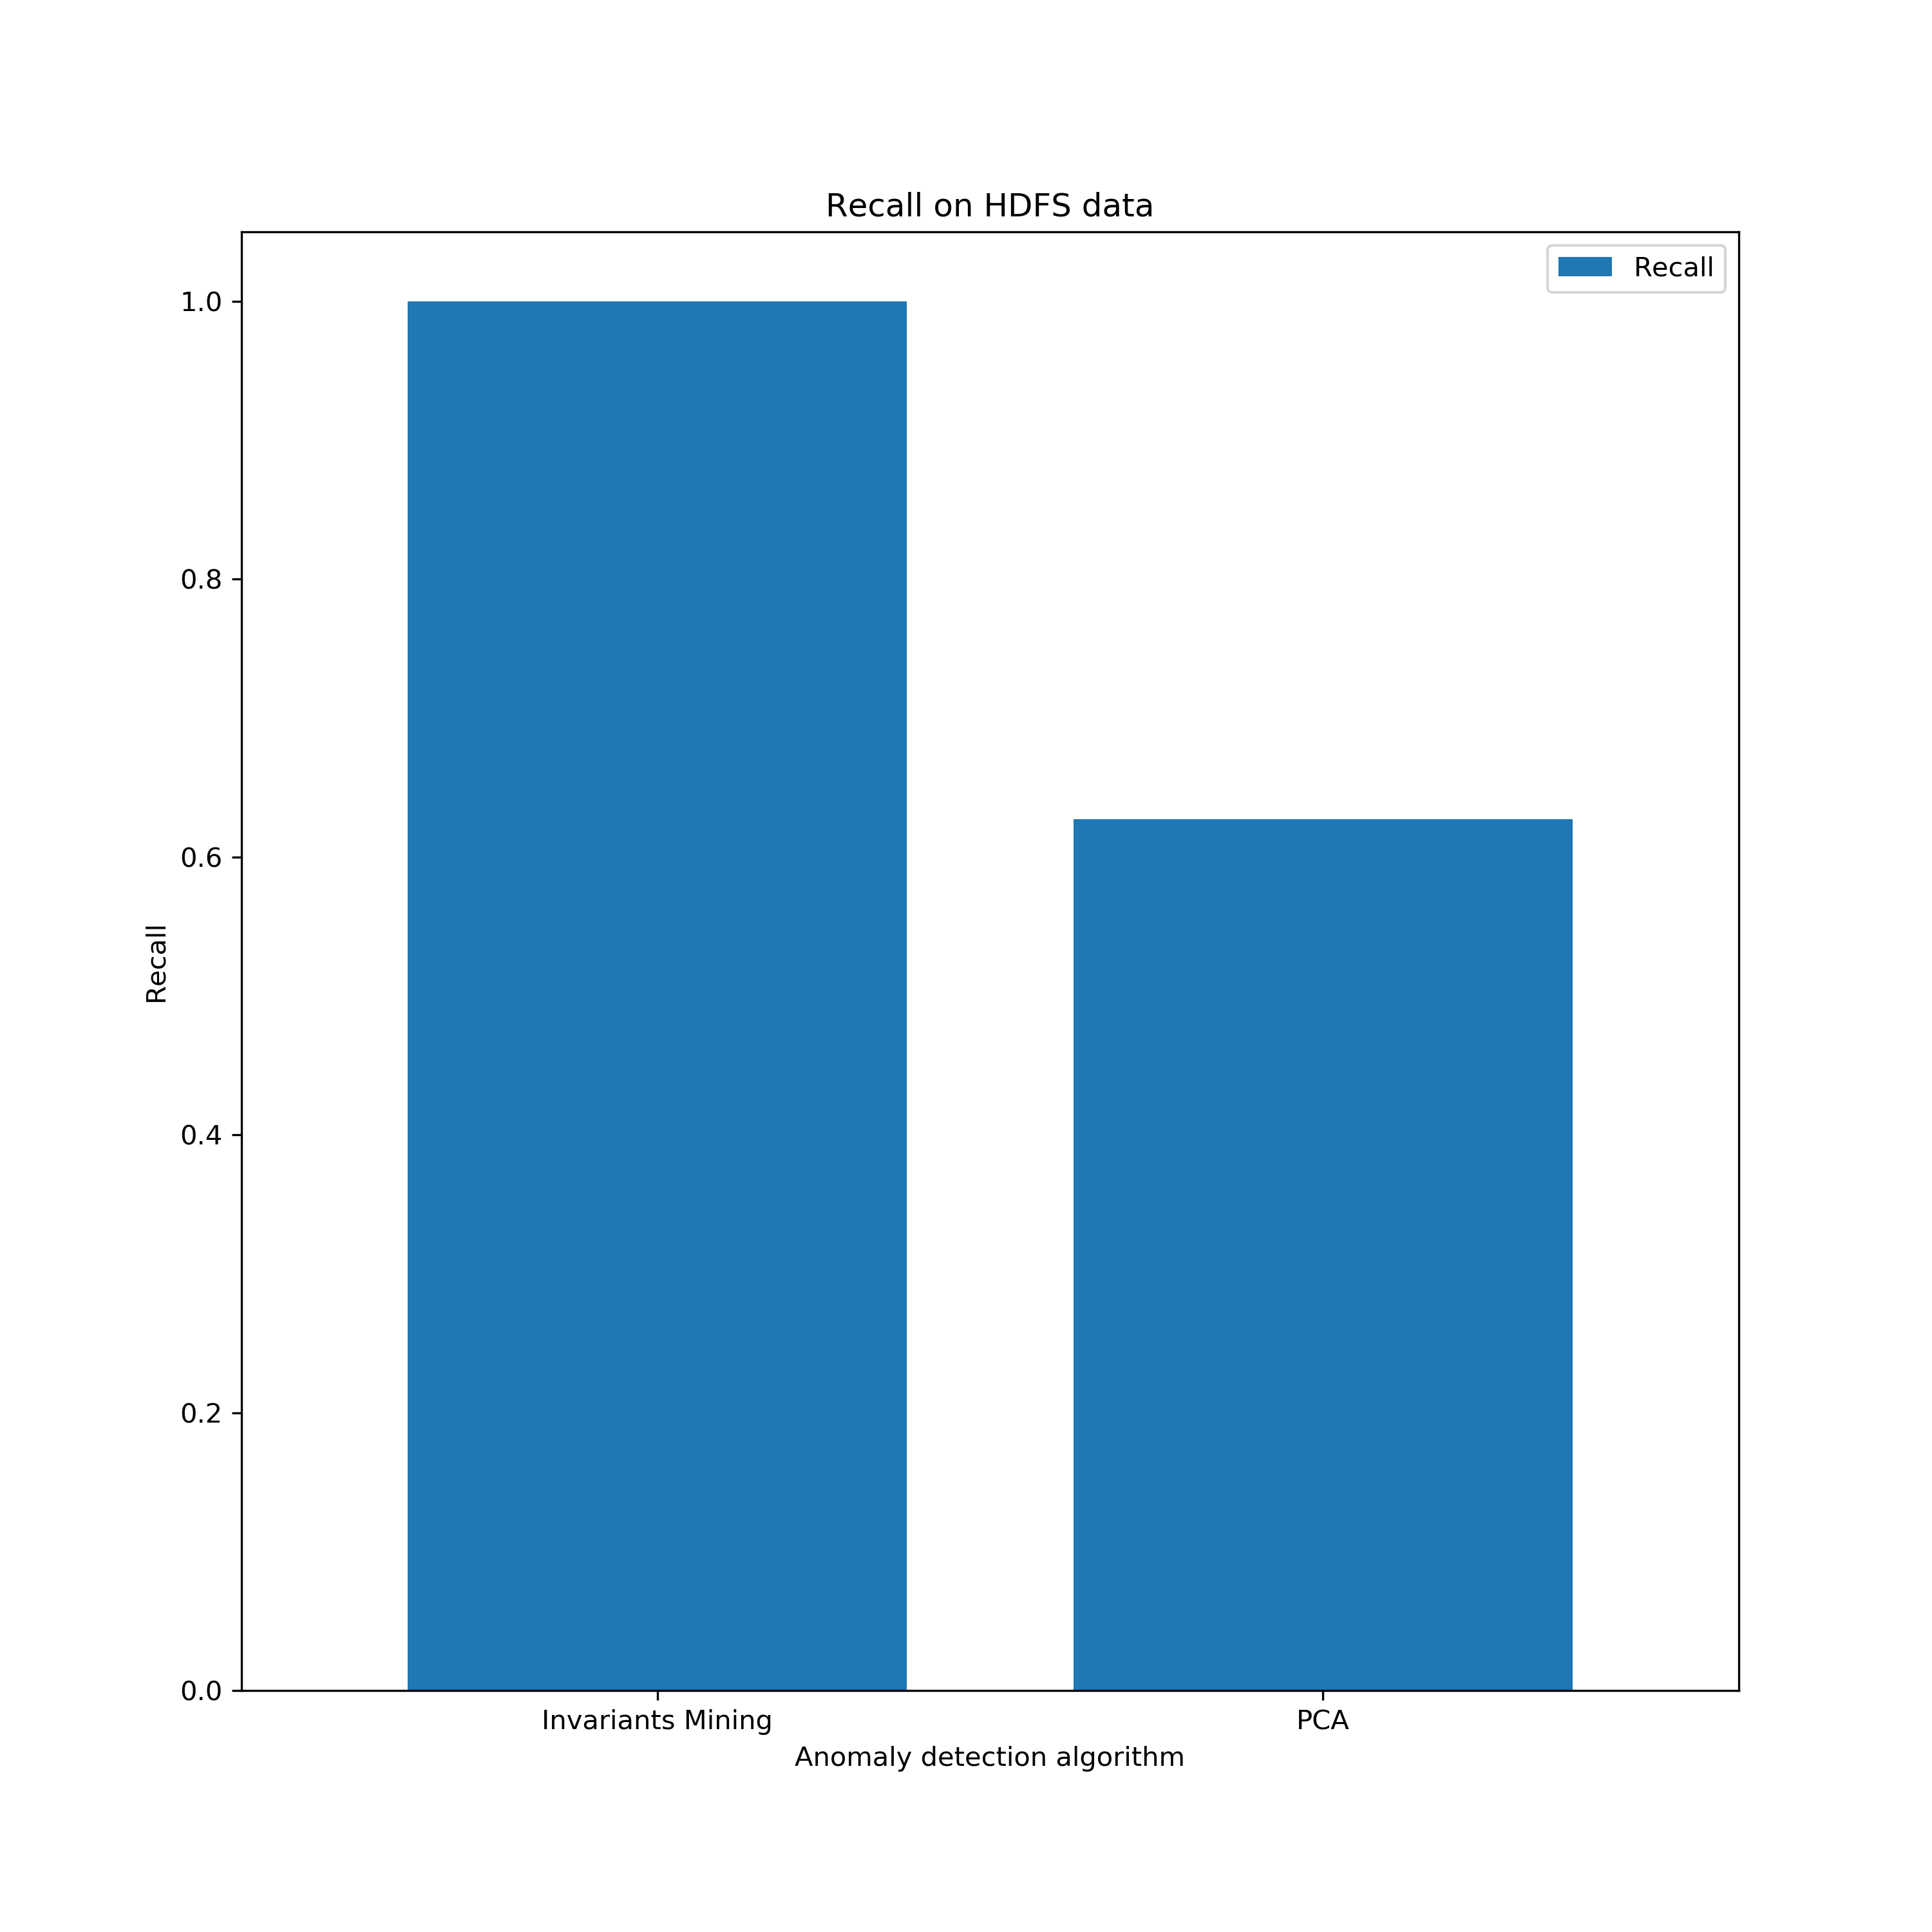
\includegraphics[width=1.3\textwidth]{Figures/Recall_2}
			
			\vspace{-0.3cm}
			\caption{Training data}
		\end{subfigure}
		\hfill
		\begin{subfigure}[H]{0.45\textwidth}
			\centering
			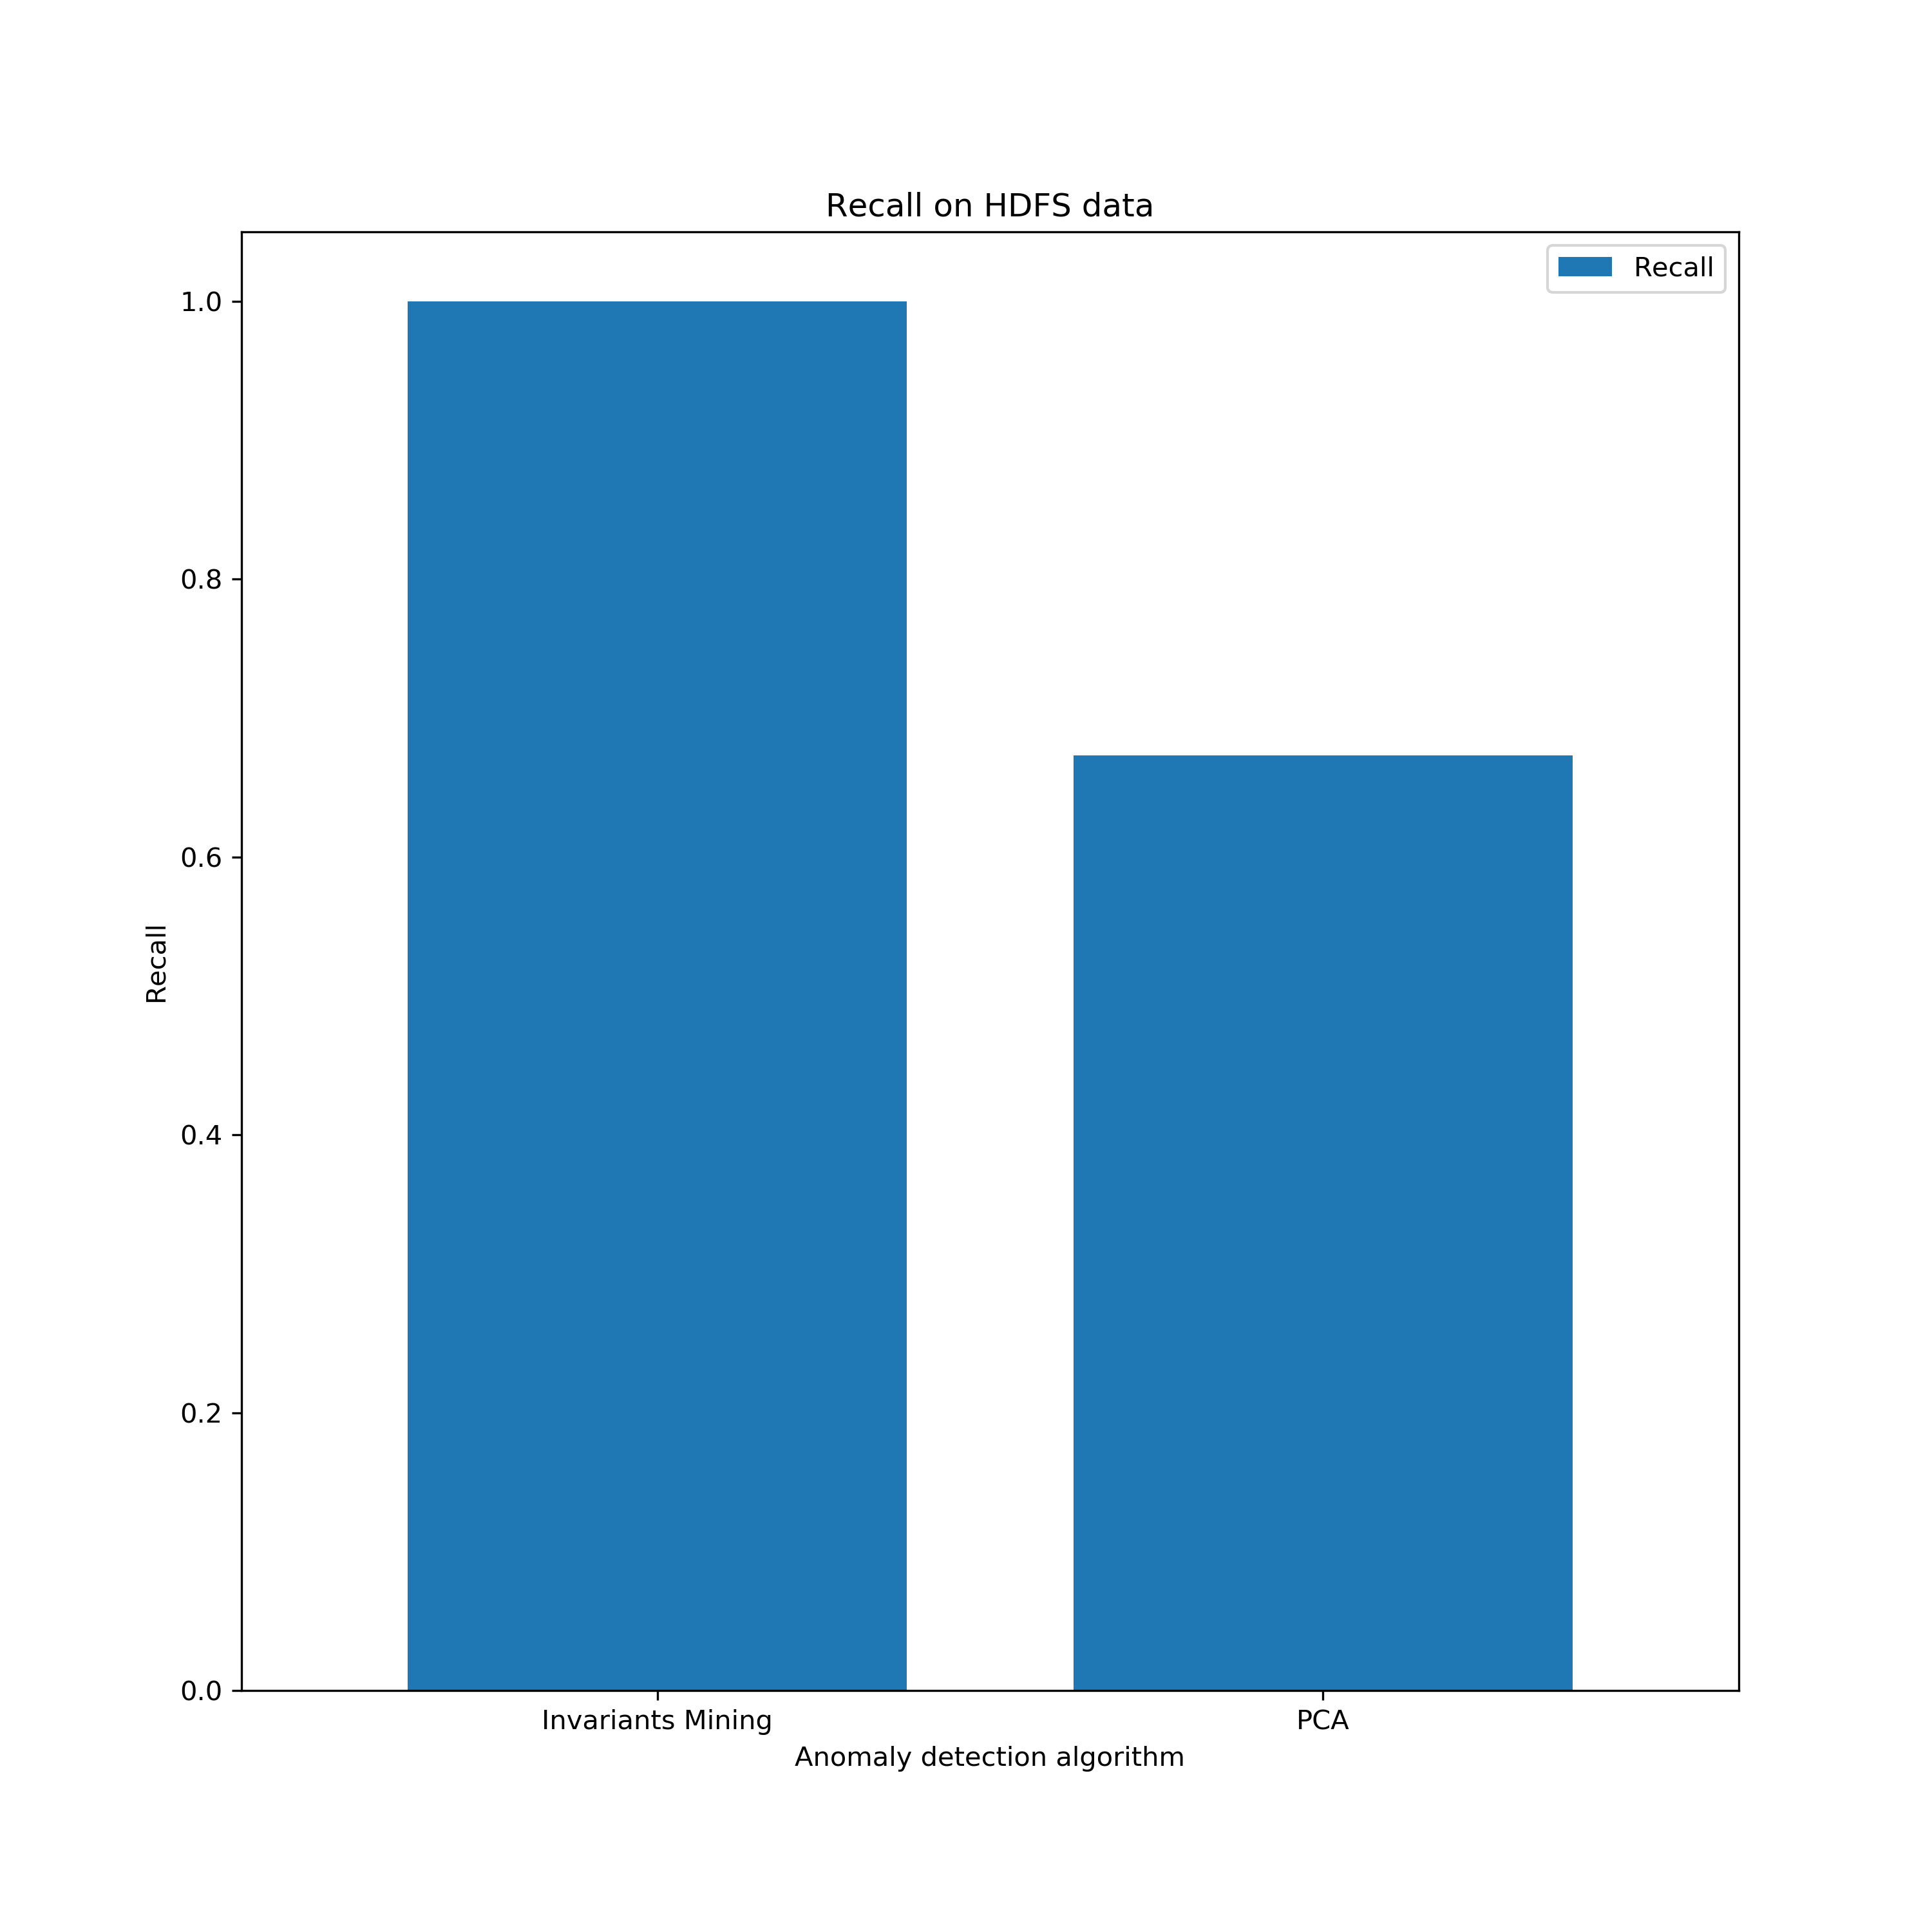
\includegraphics[width=1.3\textwidth]{Figures/Recall_2_test}
			
			\vspace{-0.3cm}
			\caption{Testing data}
		\end{subfigure}
		\vspace{-0.1cm}
		\caption{Recall evaluation results for HDFS data}
	\end{figure}

	\vspace{-0.4cm}
	\begin{figure}[H]
		\centering
		\begin{subfigure}[H]{0.45\textwidth}
			\centering
			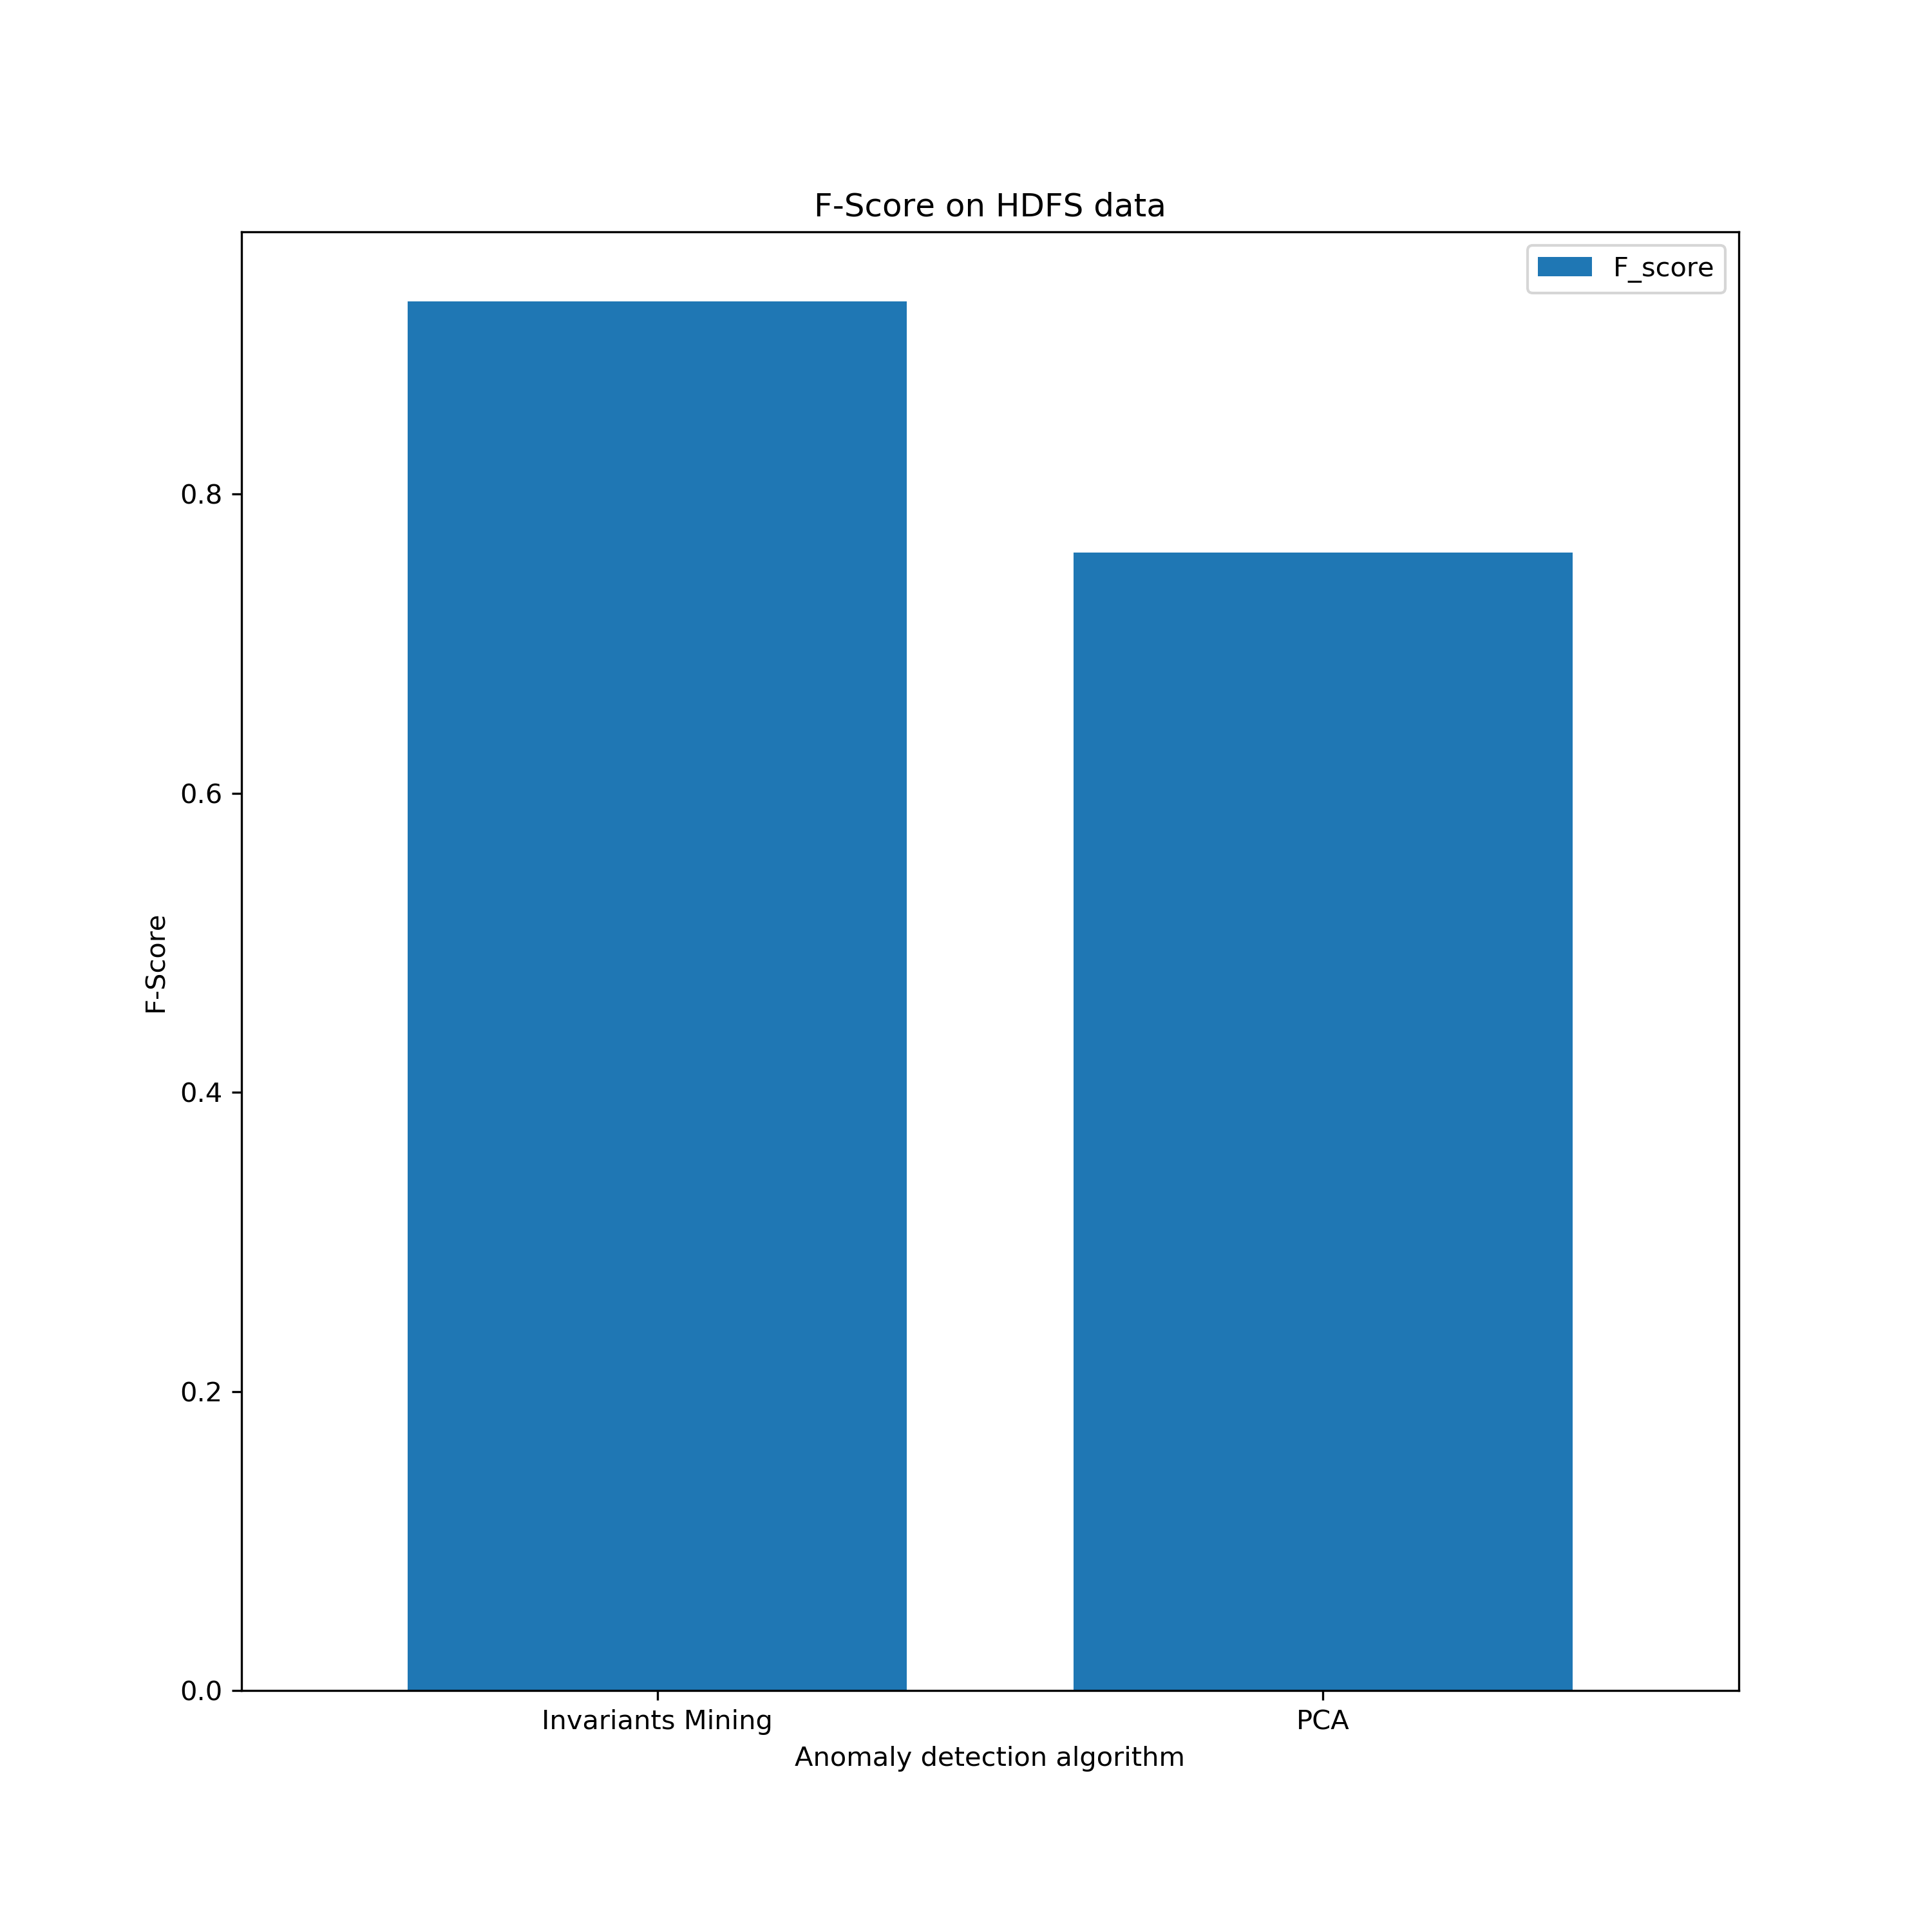
\includegraphics[width=1.3\textwidth]{Figures/F_2}
			
			\vspace{-0.3cm}
			\caption{Training data}
		\end{subfigure}
		\hfill
		\begin{subfigure}[H]{0.45\textwidth}
			\centering
			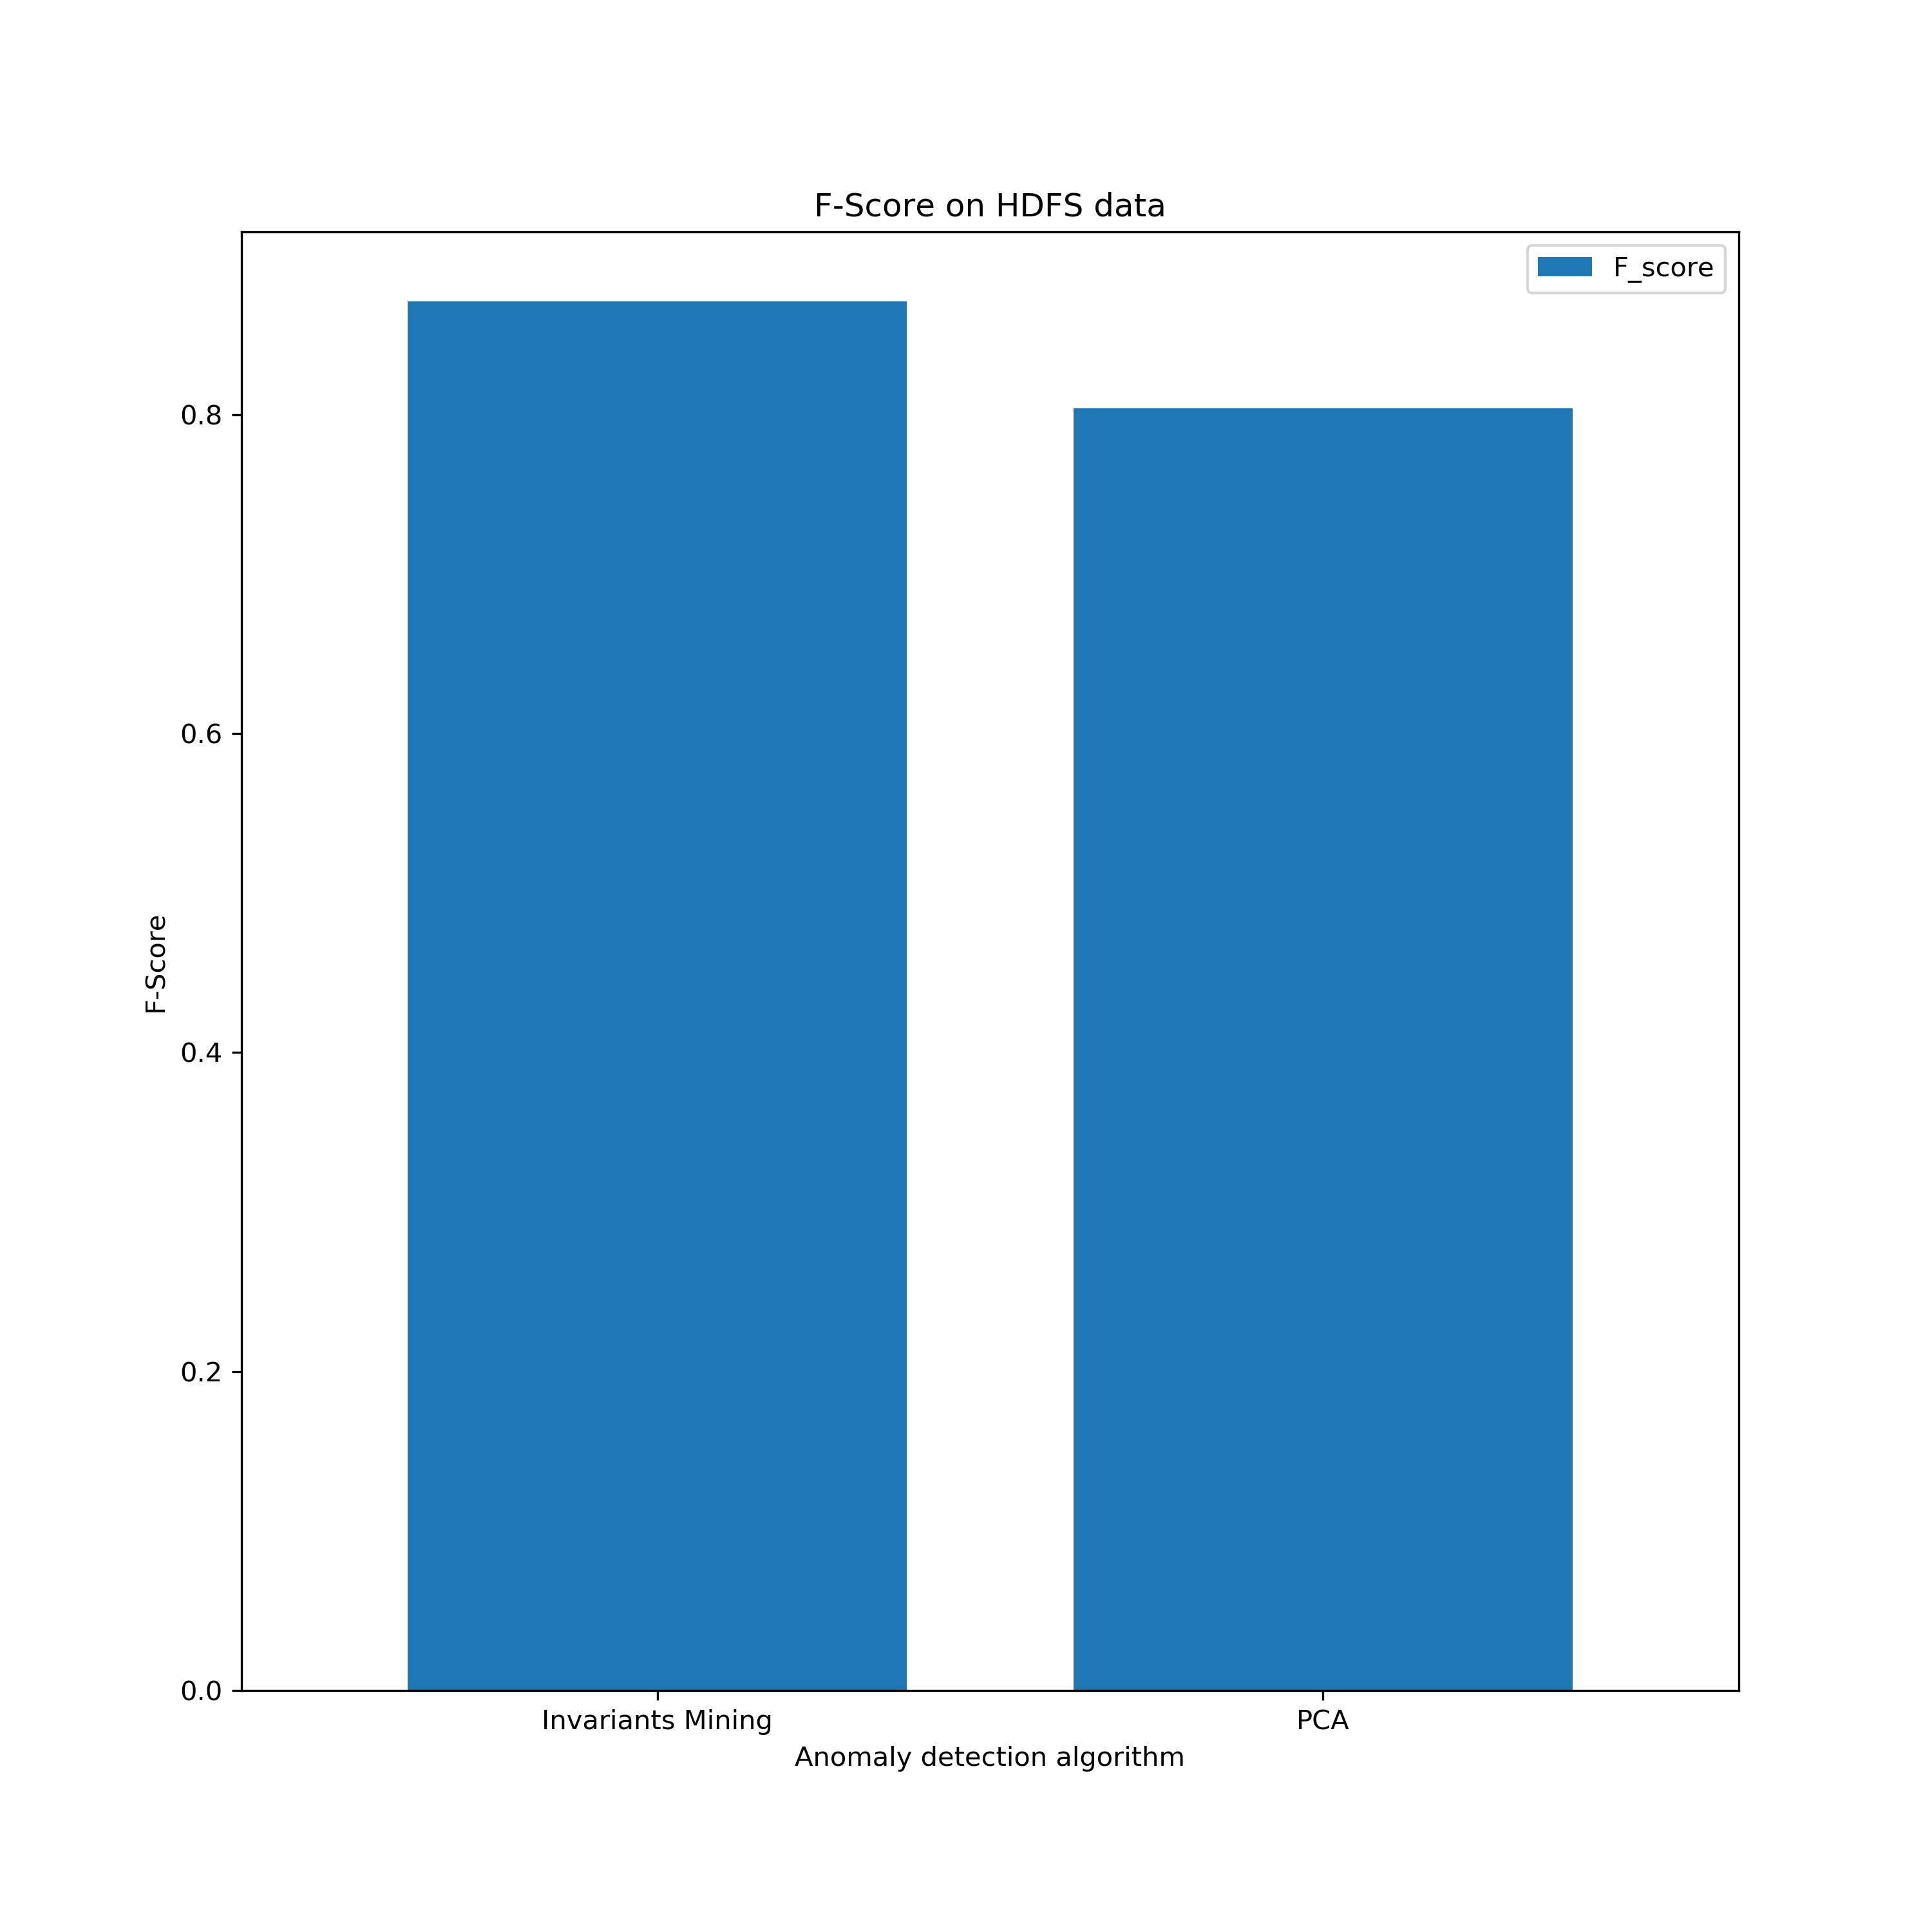
\includegraphics[width=1.3\textwidth]{Figures/F_2_test}
			
			\vspace{-0.3cm}
			\caption{Testing data}
		\end{subfigure}
		\vspace{-0.1cm}
		\caption{F-Score evaluation results for HDFS data}
	\end{figure}

	\vspace{-0.1cm}
	\noindent Based on the above figures, it is shown that PCA is able to produce slightly more precise results, with more of an advantage on the testing data; however, recall for the results of the Invariants Mining method is considerably higher than PCA, considering both training and testing data. Evidently, the F-score evaluation results demonstrate Invariants Mining's clear advantage in comparison with PCA.


	\vspace{-0.3cm}
	\begin{figure}[H]
		\centering
		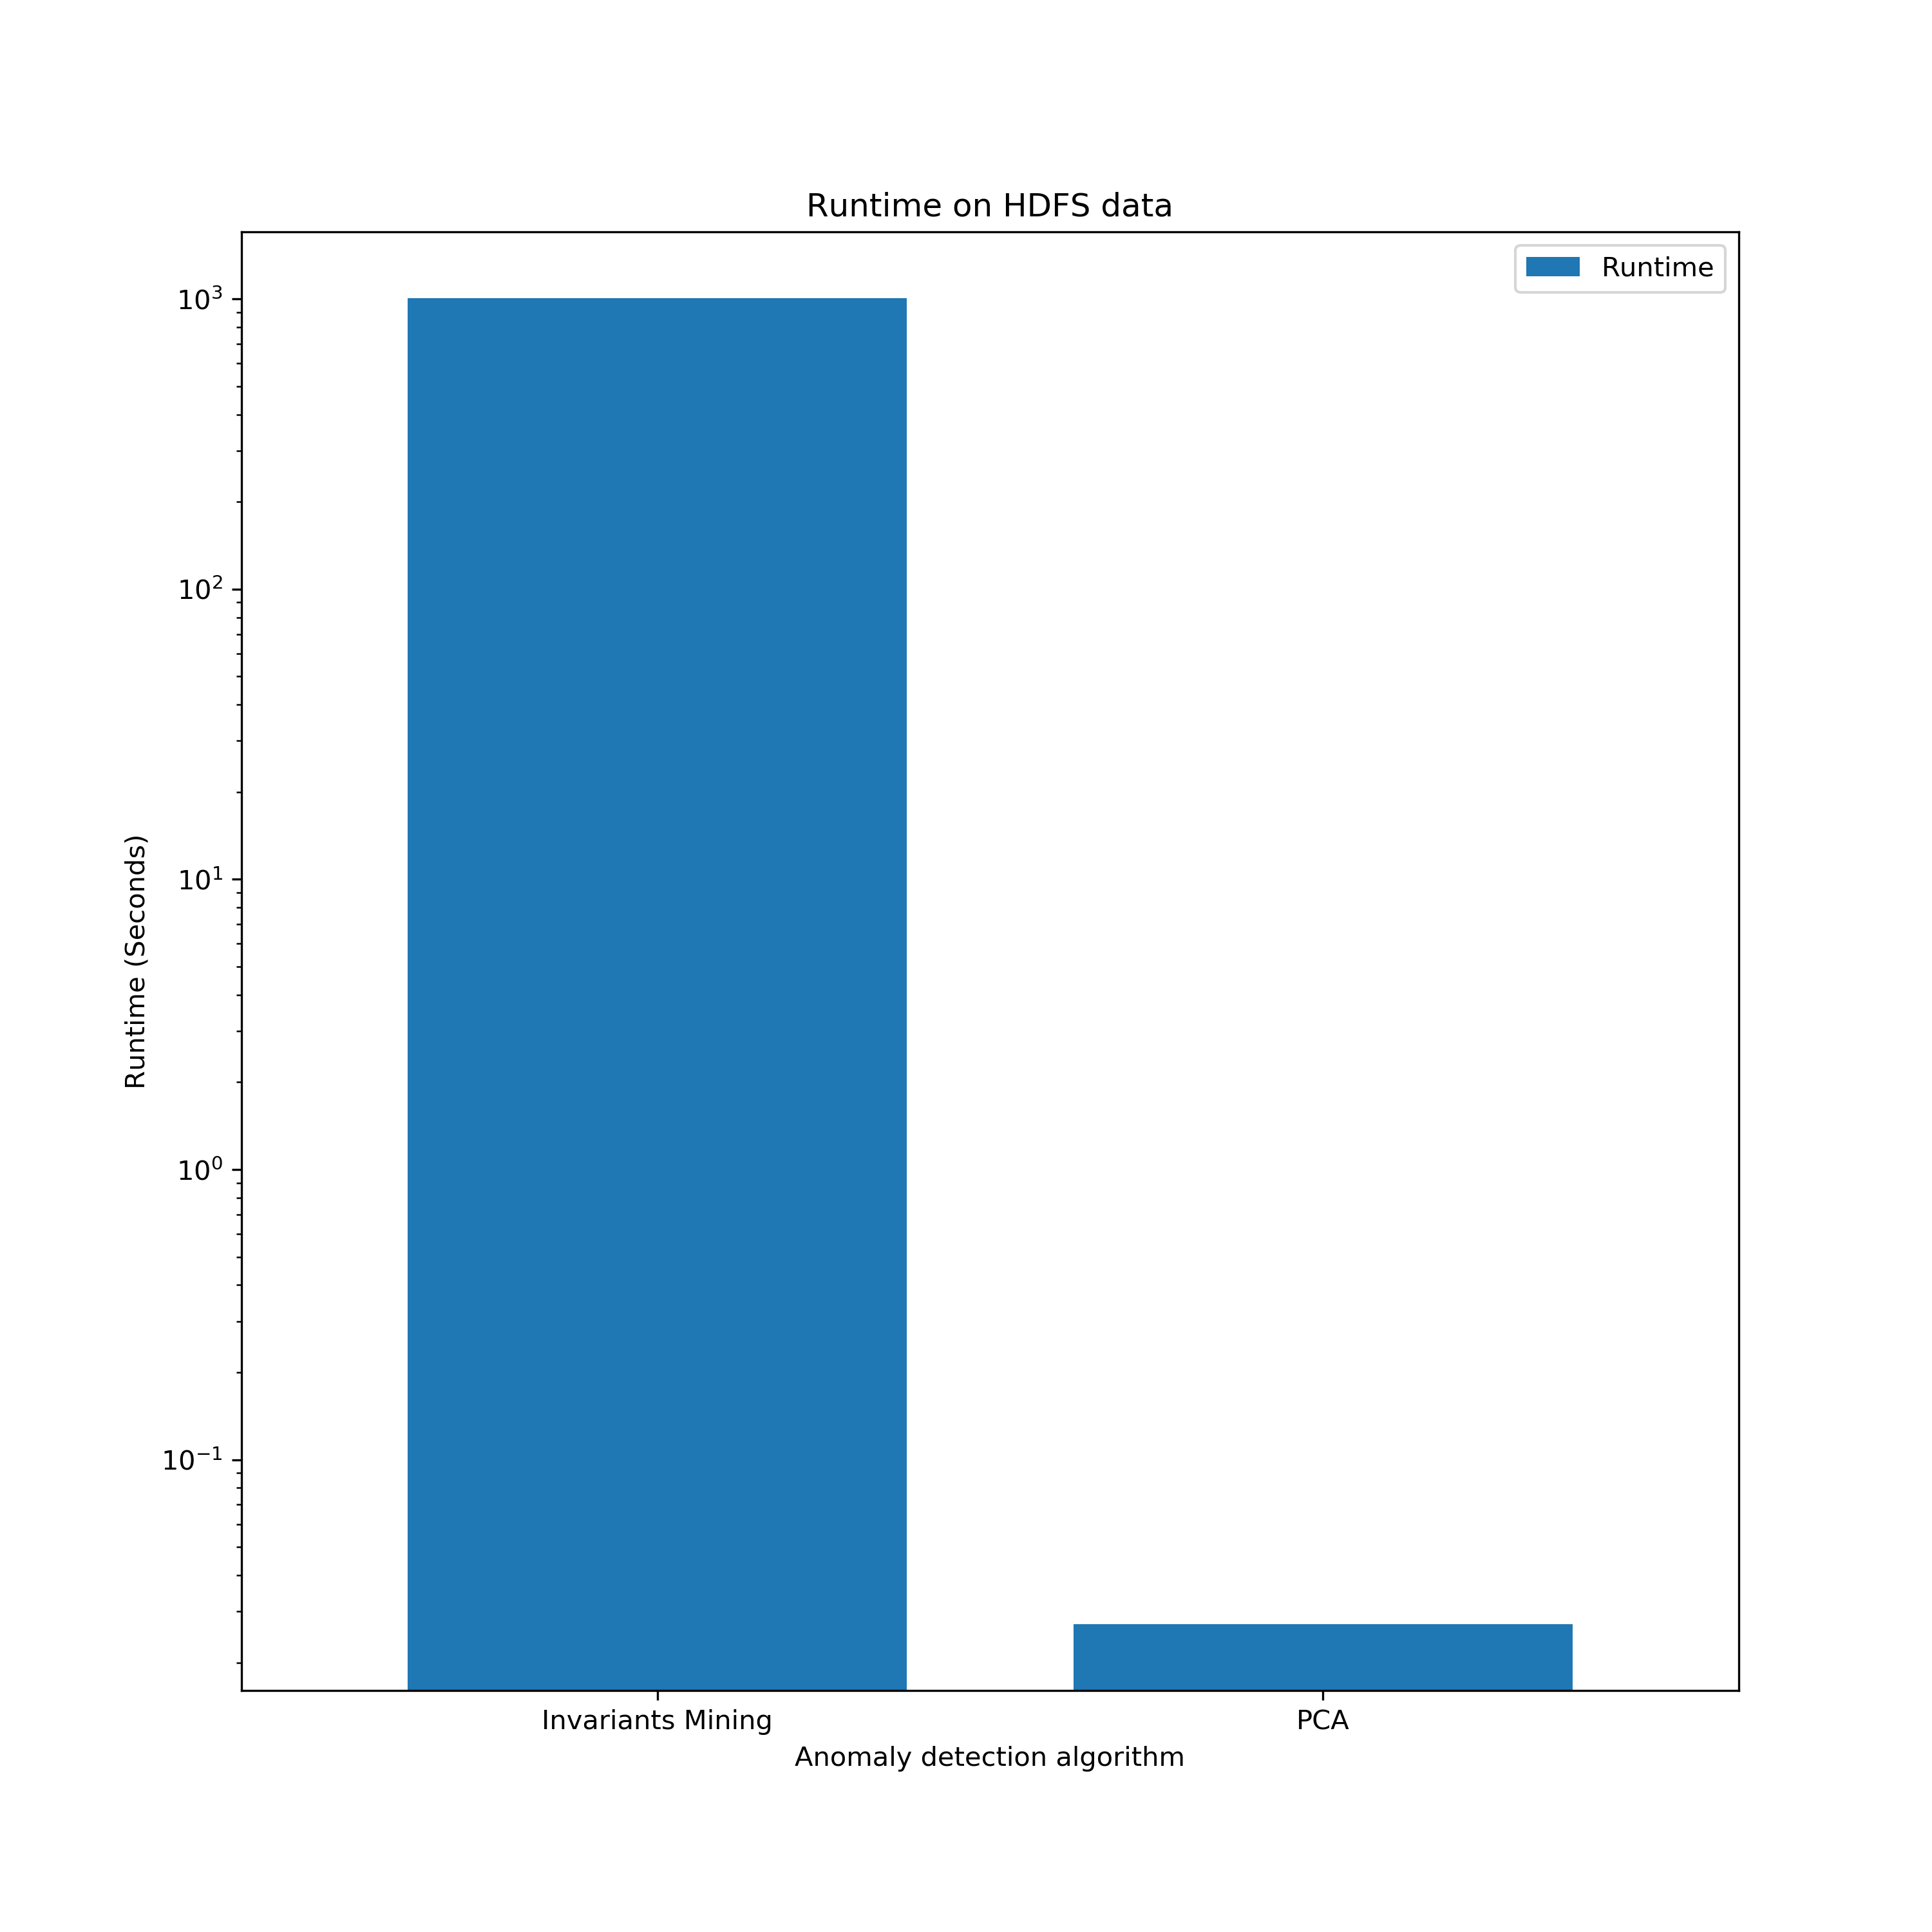
\includegraphics[width=11cm, height=8cm]{Figures/Runtime_2}
		\vspace{-0.8cm}
		
		\caption{Runtime evaluation results for HDFS data}
	\end{figure}
	
	\noindent In addition, modeling PCA is rather complex and due to its sensitivity to data, it could produce different values of accuracy depending on the provided data. However, runtime is also an important factor in evaluating these methods. The runtime comparison of these two methods is provided in Figure 8. According to this figure, it can be observed that the runtime for Invariants Mining is significantly larger (approximately $\times 10^4$) than PCA's. This is a huge drawback for Invariants mining since in real-world applications, anomalies must be detected as soon as possible in order to prevent extra costs and damages. Hence, there would be a trade-off between accuracy and runtime when choosing a model for anomaly detection: PCA for faster results and Invariants Mining for more accurate detection.
	
	\vspace{0.3cm}
	\noindent \textbf{Question:} Display three relationships. explain why, e.g., template A is “Interface *, changed state to down”, while template B is “Interface *, changed state to up”.
	
	\vspace{0.2cm}
	
	\noindent The relationships to be found must represent the normal behavior of the system. Therefore, if template A is “Interface *, changed state to down”, while template B is “Interface *, changed state to up”, then n(A) = n(B) if there are no anomalies; since according to the regular behavior of the system when there exists a log for the start of an action, there should be a corresponding log for the end of that action. More intuitively, if template A is "open window" and B is "close window", then they have to occur similar number of times if no anomalies happen. 
	
	\vspace{0.2cm}
	\noindent \textbf{Relationship 1: }n(A) = n(B)+n(C)+n(D), where
	
	\noindent Template A = writeBlock received exception java.io.IOException Interrupted receiveBlock\\
	Template B = Received block src / dest / of size $<*>$\\
	Template C = Unexpected error trying to delete block . BlockInfo not found in volumeMap\\
	Template D = BLOCK* ask to replicate to datanode(s)
	\vspace{0.1cm}
	
	\noindent Explanation: the first template shows cases in which an exception in the write block interrupts the receiveBlock. Accordingly, this exception could occur when a block is received, when there is an error while deleting a block, or when a block asks to replicate a data-node. Hence, with regular system behavior, the above equation must be met.
	
	\vspace{0.2cm}
	

	\noindent \textbf{Relationship 2: }n(A) = n(B), where
	
	\noindent Template A = writeBlock received exception java.io.IOException Interrupted receiveBlock\\
	Template B = PacketResponder 1 Exception java.net.SocketTimeoutException 60000 millis timeout while waiting for channel to be ready for read. ch java.nio. channels. SocketChannel[connected local / remote /]
	\vspace{0.1cm}
	
	\noindent Explanation: the first template shows cases in which an exception in the write block interrupts the receiveBlock. Accordingly, template B demonstrates exceptions that are raised due to lack of inputs to read (received blocks). Hence, the number of logs for these two templates must be similar if there are no anomalies.
	
	\vspace{0.2cm}
	\noindent \textbf{Relationship 3: }n(A) = n(B) = n(C), where
	
	\noindent Template A = Deleting block file $<*>$\\
	Template B = BLOCK * NameSystem.delete is added to invalidSet of\\
	Template C = BLOCK * ask to delete
	\vspace{0.1cm}

	\noindent Explanation: the first template represents the cases in which a block is being deleted. This would be the results of a block asking to delete. Accordingly, after the block is deleted, its name system would be added to the invalid set since it's no longer available. Hence, the number of logs for this three templates would be equal in normal situations.
	
	\vspace{0.4cm}
	\noindent \textbf{\Large Personal Experience, Findings, and Limitations}
	\vspace{0.3cm}
	
	\noindent Personally, I believe that this assignment overall was a little underwhelming. I believe that asking the students to search and implement some models themselves would be a much more interactive and valuable learning experience, whereas the biggest challenge of this assignment was to run the source code. Nevertheless, the content and findings of this assignment were considered to be fairly useful, especially for the upcoming group project. The tasks provided significant insight to the topic of anomaly detection, which is necessary for this course. 
	
	\noindent There were also some factors that decreased the quality of this experiment, with the main factor being system limitations. For the log parsing section, the reported results for LKE and LogSig in [1] are an average of their results during 10 runs due to their bias. However, due to the system limitations, this task required a significant amount of time and therefore, the reported values are the average of five runs of the LKE and LogSig models; in addition, since the IPLoM and SLCT methods didn't experience the same bias, they were only run once. Hence, I believe that providing students with servers for this task could be highly beneficial.
	
	\vspace{0.4cm}
	\noindent \textbf{\Large Conclusion}
	\vspace{0.3cm}
	
	\noindent In this assignment, the processes involved in any anomaly detection framework, log parsing, feature extraction, and anomaly detection, were investigated and analyzed via multiple state-of-the-art algorithms. Accordingly the obtained results were evaluated on a set of given metrics and the advantages and disadvantages of the studied methods were discussed. In conclusion, this assignment is considered as a valuable learning opportunity as encourages students to conduct the required research to a certain level in order to complete the given tasks and allows the students to acknowledge the core part of this course: anomaly detection. 
	
	\noindent \textbf{\Large References}
	\vspace{0.5cm}
	
	\noindent[1] He P, Zhu J, He S, et al. An Evaluation Study on Log Parsing and Its Use in Log Mining, Ieee/ifip International Conference on Dependable Systems and Networks. IEEE Computer Society, 2016:654-661.
	
	\vspace{0.2cm}
	\noindent[2] https://nlp.stanford.edu/IR-book/html/htmledition/evaluation-of-clustering-1.html
	
	\vspace{0.2cm}
	\noindent[3] He S, Zhu J, He P, et al. Experience Report: System Log Analysis for Anomaly Detection, IEEE, ISSRE 2016.
	
	\vspace{0.2cm}
	\noindent [4] logpai logparser [Source code]. https://github.com/logpai/logparser
	
	\vspace{0.2cm}
	\noindent [5] logpai loglizer [Source code]. https://github.com/logpai/loglizer
	
	\newpage
	\noindent \textbf{\huge Appendix}
	
	\vspace{0.5cm}
	\noindent The discovered invariants relationships are as follows:
	\vspace{0.3cm}
	
	\noindent BLOCK* NameSystem.addStoredBlock Redundant addStoredBlock request received for on size $<*>$ = Starting thread to transfer block to
	
	\noindent BLOCK* NameSystem.addStoredBlock Redundant addStoredBlock request received for on size $<*>$ = Received block src / dest / of size $<*>$
	
	\noindent BLOCK* NameSystem.addStoredBlock Redundant addStoredBlock request received for on size $<*>$ = Receiving empty packet for block
	
	\noindent BLOCK* NameSystem.addStoredBlock Redundant addStoredBlock request received for on size $<*>$ = Unexpected error trying to delete block . BlockInfo not found in volumeMap.
	
	\noindent BLOCK* NameSystem.addStoredBlock Redundant addStoredBlock request received for on size $<*>$ = BLOCK* ask to replicate to datanode(s)
	
	\noindent BLOCK* NameSystem.addStoredBlock Redundant addStoredBlock request received for on size $<*>$ = BLOCK* NameSystem.addStoredBlock addStoredBlock request received for on size $<*>$ But it does not belong to any file.
	
	\noindent Starting thread to transfer block to = PacketResponder 1 Exception java.net .Socket TimeoutException 60000 millis timeout while waiting for channel to be ready for read. ch java.nio.channels.SocketChannel[connected local / remote /]
	
	\noindent Starting thread to transfer block to = writeBlock received exception java.io.IOException Interrupted receiveBlock
	Starting thread to transfer block to = writeBlock received exception $<*>$ $<*>$ $<*>$ $<*>$ $<*>$
	
	\noindent Starting thread to transfer block to = BLOCK* Removing block from neededReplications as it does not belong to any file.
	
	\noindent Starting thread to transfer block to = writeBlock received exception java.net. SocketTimeoutException $<*>$ millis timeout while waiting for channel to be ready for $<*>$ ch java.nio.channels. SocketChannel[connected local / remote /]
	
	\noindent Starting thread to transfer block to = Exception in receiveBlock for block $<*>$
	
	\noindent Starting thread to transfer block to = writeBlock received exception java.io.IOException Could not read from stream
	
	\noindent Starting thread to transfer block to = Exception writing block to mirror
	
	\noindent Starting thread to transfer block to = PacketResponder $<*>$ Exception $<*>$
	
	\noindent Starting thread to transfer block to = $<*>$ $<*>$ $<*>$ java.io.IOException Broken pipe
	
	\noindent Starting thread to transfer block to = DataXceiver java.io.IOException Block is not valid.
	
	\noindent Starting thread to transfer block to = Reopen Block
	
	\noindent Starting thread to transfer block to = writeBlock received exception java.io.IOException Block is valid and cannot be written to.
	
	\noindent Starting thread to transfer block to = PacketResponder 2 Exception java.net. SocketTimeoutException 120000 millis timeout while waiting for channel to be ready for read. ch java.nio.channels. SocketChannel[connected local / remote /]
	
	\noindent Starting thread to transfer block to = Exception in receiveBlock for block java.io.IOException Broken pipe
	
	\noindent Starting thread to transfer block to = Exception in receiveBlock for block java.net. SocketTimeoutException $<*>$ millis timeout while waiting for channel to be ready for write. ch java.nio.channels. SocketChannel[connected local / remote /]
	
	\noindent Starting thread to transfer block to = $<*>$ $<*>$ $<*>$ $<*>$ $<*>$ java.io.IOException Connection reset by peer
	Starting thread to transfer block to = PendingReplicationMonitor timed out block
	
	\noindent Starting thread to transfer block to = PacketResponder $<*>$ Exception java.io.IOException $<*>$ $<*>$ $<*>$ $<*>$
	
	\noindent Starting thread to transfer block to = Adding an already existing block
	
	\noindent Starting thread to transfer block to = Changing block file offset of block from 0 to $<*>$ meta file offset to $<*>$
	
	\noindent Starting thread to transfer block to = writeBlock received exception $<*>$
	
	\noindent Starting thread to transfer block to = Exception in receiveBlock for block java.io. InterruptedIOException Interruped while waiting for IO on channel java.nio.channels. SocketChannel[connected local / remote /]. $<*>$ millis timeout left.
	
	\noindent Starting thread to transfer block to = PacketResponder 1 Exception java.io. InterruptedIOException Interruped while waiting for IO on channel java.nio.channels. SocketChannel[closed]. $<*>$ millis timeout left.
	
	\noindent Starting thread to transfer block to = DataXceiver java.io.IOException Block is valid and cannot be written to.
	
	\noindent Starting thread to transfer block to = $<*>$ $<*>$ $<*>$ java.io. InterruptedIOException Interruped while waiting for IO on channel java.nio.channels. SocketChannel[connected local / remote /]. $<*>$ millis timeout left.
	
	\noindent Deleting block file $<*>$ = BLOCK* NameSystem.delete is added to invalidSet of
	
	\noindent Deleting block file $<*>$ = BLOCK* ask to delete
	
	\noindent PacketResponder 1 Exception java.net.SocketTimeoutException 60000 millis timeout while waiting for channel to be ready for read. ch java.nio.channels. SocketChannel[connected local / remote /] = Received block src / dest / of size $<*>$
	
	\noindent PacketResponder 1 Exception java.net.SocketTimeoutException 60000 millis timeout while waiting for channel to be ready for read. ch 
	java.nio.channels. SocketChannel[connected local / remote /] = Unexpected error trying to delete block . BlockInfo not found in volumeMap.
	
	\noindent PacketResponder 1 Exception java.net.SocketTimeoutException 60000 millis timeout while waiting for channel to be ready for read. ch java.nio.channels. SocketChannel[connected local / remote /] = BLOCK* ask to replicate to datanode(s)
	
	\noindent writeBlock received exception java.io.IOException Interrupted receiveBlock = Received block src / dest / of size $<*>$
	
	\noindent writeBlock received exception java.io.IOException Interrupted receiveBlock = Unexpected error trying to delete block . BlockInfo not found in volumeMap.
	
	\noindent writeBlock received exception java.io.IOException Interrupted receiveBlock = BLOCK* ask to replicate to datanode(s)
	
\end{document}